\documentclass[11pt,]{article}
\usepackage{lmodern}
\usepackage{amssymb,amsmath}
\usepackage{ifxetex,ifluatex}
\usepackage{fixltx2e} % provides \textsubscript
\ifnum 0\ifxetex 1\fi\ifluatex 1\fi=0 % if pdftex
  \usepackage[T1]{fontenc}
  \usepackage[utf8]{inputenc}
\else % if luatex or xelatex
  \ifxetex
    \usepackage{mathspec}
    \usepackage{xltxtra,xunicode}
  \else
    \usepackage{fontspec}
  \fi
  \defaultfontfeatures{Mapping=tex-text,Scale=MatchLowercase}
  \newcommand{\euro}{€}
\fi
% use upquote if available, for straight quotes in verbatim environments
\IfFileExists{upquote.sty}{\usepackage{upquote}}{}
% use microtype if available
\IfFileExists{microtype.sty}{%
\usepackage{microtype}
\UseMicrotypeSet[protrusion]{basicmath} % disable protrusion for tt fonts
}{}
\usepackage[margin=1in]{geometry}
\usepackage{color}
\usepackage{fancyvrb}
\newcommand{\VerbBar}{|}
\newcommand{\VERB}{\Verb[commandchars=\\\{\}]}
\DefineVerbatimEnvironment{Highlighting}{Verbatim}{commandchars=\\\{\}}
% Add ',fontsize=\small' for more characters per line
\usepackage{framed}
\definecolor{shadecolor}{RGB}{248,248,248}
\newenvironment{Shaded}{\begin{snugshade}}{\end{snugshade}}
\newcommand{\KeywordTok}[1]{\textcolor[rgb]{0.13,0.29,0.53}{\textbf{{#1}}}}
\newcommand{\DataTypeTok}[1]{\textcolor[rgb]{0.13,0.29,0.53}{{#1}}}
\newcommand{\DecValTok}[1]{\textcolor[rgb]{0.00,0.00,0.81}{{#1}}}
\newcommand{\BaseNTok}[1]{\textcolor[rgb]{0.00,0.00,0.81}{{#1}}}
\newcommand{\FloatTok}[1]{\textcolor[rgb]{0.00,0.00,0.81}{{#1}}}
\newcommand{\CharTok}[1]{\textcolor[rgb]{0.31,0.60,0.02}{{#1}}}
\newcommand{\StringTok}[1]{\textcolor[rgb]{0.31,0.60,0.02}{{#1}}}
\newcommand{\CommentTok}[1]{\textcolor[rgb]{0.56,0.35,0.01}{\textit{{#1}}}}
\newcommand{\OtherTok}[1]{\textcolor[rgb]{0.56,0.35,0.01}{{#1}}}
\newcommand{\AlertTok}[1]{\textcolor[rgb]{0.94,0.16,0.16}{{#1}}}
\newcommand{\FunctionTok}[1]{\textcolor[rgb]{0.00,0.00,0.00}{{#1}}}
\newcommand{\RegionMarkerTok}[1]{{#1}}
\newcommand{\ErrorTok}[1]{\textbf{{#1}}}
\newcommand{\NormalTok}[1]{{#1}}
\usepackage{longtable,booktabs}
\usepackage{graphicx}
\makeatletter
\def\maxwidth{\ifdim\Gin@nat@width>\linewidth\linewidth\else\Gin@nat@width\fi}
\def\maxheight{\ifdim\Gin@nat@height>\textheight\textheight\else\Gin@nat@height\fi}
\makeatother
% Scale images if necessary, so that they will not overflow the page
% margins by default, and it is still possible to overwrite the defaults
% using explicit options in \includegraphics[width, height, ...]{}
\setkeys{Gin}{width=\maxwidth,height=\maxheight,keepaspectratio}
\ifxetex
  \usepackage[setpagesize=false, % page size defined by xetex
              unicode=false, % unicode breaks when used with xetex
              xetex]{hyperref}
\else
  \usepackage[unicode=true]{hyperref}
\fi
\hypersetup{breaklinks=true,
            bookmarks=true,
            pdfauthor={},
            pdftitle={Are environmental and geographic effective surrogates for genetic variation in conservation planning?},
            colorlinks=true,
            citecolor=blue,
            urlcolor=blue,
            linkcolor=magenta,
            pdfborder={0 0 0}}
\urlstyle{same}  % don't use monospace font for urls
\setlength{\parindent}{0pt}
\setlength{\parskip}{6pt plus 2pt minus 1pt}
\setlength{\emergencystretch}{3em}  % prevent overfull lines
\setcounter{secnumdepth}{0}

%%% Use protect on footnotes to avoid problems with footnotes in titles
\let\rmarkdownfootnote\footnote%
\def\footnote{\protect\rmarkdownfootnote}

%%% Change title format to be more compact
\usepackage{titling}

% Create subtitle command for use in maketitle
\newcommand{\subtitle}[1]{
  \posttitle{
    \begin{center}\large#1\end{center}
    }
}

\setlength{\droptitle}{-2em}
  \title{Are environmental and geographic effective surrogates for genetic
variation in conservation planning?}
  \pretitle{\vspace{\droptitle}\centering\huge}
  \posttitle{\par}
  \author{Jeffrey O. Hanson$^1$, Jonathan R. Rhodes$^2$, Cynthia Riginos$^2$, Hugh
P. Possingham$^1$, Richard A. Fuller$^1$\\$^1$School of Biological
Sciences, The University of Queensland, Brisbane, QLD,
Australia\\$^2$School of Geography, Planning and Environmental
Management, The University of Queensland, Brisbane, QLD,
Australia\\Correspondance should be addressed to
\href{mailto:jeffrey.hanson@uqconnect.edu.au}{jeffrey.hanson@uqconnect.edu.au}}
  \preauthor{\centering\large\emph}
  \postauthor{\par}
  \predate{\centering\large\emph}
  \postdate{\par}
  \date{13 December 2015}

% load packages
\usepackage{amsmath,amsfonts,float,makecell,titletoc,tocloft,titlesec,natbib}
\usepackage[T1]{fontenc}
\usepackage{lmodern}
\usepackage[utf8]{inputenc}

% format captions
\usepackage[labelfont={small,bf}, labelsep=space, font={small}]{caption}

% format headings
\titleformat{\subsection}
{\normalfont\Large\bfseries}{\thesubsection}{1em}{}
\titleformat{\subsubsection}
{\normalfont\large\bfseries}{\thesubsubsection}{1em}{}
\titleformat{\paragraph}
{\normalfont\normalsize\bfseries}{\theparagraph}{1em}{}
\titleformat{\subparagraph}
{\normalfont\normalsize\itshape}{\thesubparagraph}{1em}{}

\titlespacing\paragraph{0pt}{12pt plus 4pt minus 2pt}{+0pt plus 2pt minus 2pt}
\titlespacing{\subparagraph}{0pt}{6pt plus 4pt minus 2pt}{+0pt plus 2pt minus 2pt}

% format toc
\renewcommand\cftsubsecfont{\normalfont\normalsize\bfseries}
% \renewcommand\cftsubsubsecfont{\normalfont\normalsize\bfseries}
% \renewcommand\cftparafont{\normalfont\normalsize\bfseries}
% \renewcommand\cftsubparafont{\normalfont\normalsize\itshape}

% make figures static
\let\origfigure\figure
\let\endorigfigure\endfigure
\renewenvironment{figure}[1][2] {
	\expandafter\origfigure\expandafter[H]
} {
	\endorigfigure
}


\begin{document}

\maketitle

\begin{abstract}
Insert abstract here.
\end{abstract}

{
\hypersetup{linkcolor=black}
\setcounter{tocdepth}{5}
\tableofcontents
}
\subsection{Introduction}\label{introduction}

\subsection{Methods}\label{methods}

\subsubsection{Study area}\label{study-area}

To address the aims of this study, we utilized species distribution and
genomic data collected by the IntraBioDiv project (Figure S1; Meirmans
\emph{et al.} 2011). As part of this project, data for 27 alpine plant
species were collected across the European Alps using a regular grid
(22.3 km $\times$ 25 km; see Gugerli \emph{et al.} 2008 for
methodological details). In every second cell, plant samples were
collected from three individiduals for each species present inside the
cell. Samples were genotyped using amplified fragment length
polymorphisms (AFLP; Vos \emph{et al.} 1995). Matrices denoting the
presence/absence of polymorphisms at loci were consutrcted independently
for each species. This dataset was well suited for the purposes of this
study, because it provides spatially explicit genomic data for a
multitude of species. Additionally, the study area spans across
broad-scale environmental gradients--ranging from lowlands to snow-caped
peaks--that have been found to correlate with genetic variation for some
of these species {[}{]}.

\subsubsection{Surrogate data}\label{surrogate-data}

We explored the effectiveness of environmental and geographic
surrogates. To describe variation in the location of each grid, we
projected the grids to an equal-area coordinate system (ESRI:102014) and
determined the centroid of each cell. To describe the climatic variation
among each cell, we obtained twenty-one bioclimatic variables (Hijmans
\emph{et al.} 2005). These layers were clipped to the extent of the grid
and subject to a principle components analysis (PCA; Table S1). The
first two principle components (PCs) cumulatively explained 97.2\% of
the variation and were used to generate two new layers. The average
value of each PC layer in each grid was used to characterise the
climatic conditions in the grid cell (Figure S2).

\subsubsection{Outlier locus detection}\label{outlier-locus-detection}

To investigate the effectiveness of the surrogates for adaptive and
neutral genetic variation, we first identifed which of the sampled loci
for each species for each species were under selection. We used an
outlier locus detection method (evaluated in P{é}rez-Figueroa \emph{et
al.} 2010) to avoid circularity issues. The basic premise underpinning
this method is that neutral loci are expected to have a specific level
of variation among populations ($F_{st}$), and loci that deviate from
this expectation are under selection. Previously, Bothwell \emph{et al.}
(2013) applied such detection methods to one of the species
(\emph{Getiana nivalis}) in this dataset. Here, we applied their methods
to each of the twenty-seven species in the dataset.

Breifly, we grouped individuals into genetic lineages (Figure S2). The
purpose of this step was to avoid confounding variation between
populations with due to genetic history with variation attributed to
selection pressures. We used the Bayesian clustering method implemented
in Structure (version 2.3.4) assuming admixture and an independent
alleles model. For each species, we identified the most plausible number
of populations (K = 1--10; 4 runs for each K; model with lowest mean
posterior negative log likelihood; Figure S3), and estimated the
probability that each individual belonged to each population (10
burn-in; 10 iterations). Individuals with $\geq 0.75$ probability of
belonging to a single population were assigned accordingly (Figure S4),
and used for subseqent detection methods.

We used Bayescan (version 2.1; Foll and Gaggiotti 2008) to identify the
sampled loci under selection for each species (Table S2). For each
species, Bayescan was run using the population memberships identified
using Structure (1:1 prior odds, 3 pilot runs, and 10 iterations thinned
by 1 iterations with a 40 burn-in). Following guidelines in the Bayescan
manual, we omitted loci where the global frequency of the minor allele
was $\geq$ 0.05 to avoid false-positives. To ensure convergence, we ran
2 replicates per species using a false discovery rate (FDR) $\leq 0.5$.

After classifying the loci as adaptive or neutral for each species, we
mapped the main gradients of adaptive and/or neutral genetic variation
for each species (Figures S4--S29). For each species, we used Gower
distances to express the difference in adaptive and/or neutral
polymorphisms between individuals (using the cluster R package; Maechler
\emph{et al.} 2015). These distances were subject to a non metric
multi-dimensional scaling analysis (implemented in the vegan R package
using K=2 and 2 random starts; Table S3; Oksanen \emph{et al.} 2015).
The ordinated variables were then associated with the grid cells were
each species was sampled.

\subsubsection{Prioritisations}\label{prioritisations}

\subsection{Results}\label{results}

\subsubsection{Single species
prioritisations}\label{single-species-prioritisations}

\begin{Shaded}
\begin{Highlighting}[]
\CommentTok{# prepare data for plotting}
\NormalTok{single.spp.PDF <-}\StringTok{ }\KeywordTok{expand.grid}\NormalTok{(}
    \DataTypeTok{Prioritisation=}\KeywordTok{unique}\NormalTok{(single.spp.SDF$Prioritisation),}
    \DataTypeTok{Metric=}\KeywordTok{unique}\NormalTok{(single.spp.SDF$Metric))}
\NormalTok{single.spp.PDF <-}\StringTok{ }\KeywordTok{cbind}\NormalTok{(single.spp.PDF,}
    \KeywordTok{as.data.frame}\NormalTok{(}\KeywordTok{predict}\NormalTok{(single.spp.GLM, single.spp.PDF,}
        \DataTypeTok{type=}\StringTok{'response'}\NormalTok{, }\DataTypeTok{se.fit=}\OtherTok{TRUE}\NormalTok{))) %>%}
\StringTok{    }\KeywordTok{mutate}\NormalTok{(}\DataTypeTok{lower=}\NormalTok{fit-se.fit, }\DataTypeTok{upper=}\NormalTok{fit+se.fit,}
        \DataTypeTok{letters=}\KeywordTok{toupper}\NormalTok{(}\KeywordTok{cld}\NormalTok{(single.spp.MCP)$mcletters$Letters),}
        \DataTypeTok{letter_pos=}\NormalTok{upper}\FloatTok{+0.05}\NormalTok{)}
\CommentTok{# make plot}
\KeywordTok{ggplot}\NormalTok{(}\KeywordTok{aes}\NormalTok{(}\DataTypeTok{x=}\NormalTok{Metric,}\DataTypeTok{y=}\NormalTok{fit,}\DataTypeTok{fill=}\NormalTok{Prioritisation),}
    \DataTypeTok{data=}\NormalTok{single.spp.PDF) +}
\StringTok{    }\KeywordTok{geom_bar}\NormalTok{(}\DataTypeTok{position=}\KeywordTok{position_dodge}\NormalTok{(}\FloatTok{0.9}\NormalTok{),}
        \DataTypeTok{stat=}\StringTok{'identity'}\NormalTok{) +}
\StringTok{    }\KeywordTok{geom_errorbar}\NormalTok{(}
        \KeywordTok{aes}\NormalTok{(}\DataTypeTok{ymin=}\NormalTok{lower,}\DataTypeTok{ymax=}\NormalTok{upper),}
        \DataTypeTok{position=}\KeywordTok{position_dodge}\NormalTok{(}\FloatTok{0.9}\NormalTok{), }\DataTypeTok{width=}\FloatTok{0.6}\NormalTok{) +}
\StringTok{    }\KeywordTok{geom_text}\NormalTok{(}\KeywordTok{aes}\NormalTok{(}\DataTypeTok{x=}\NormalTok{Metric, }\DataTypeTok{y=}\NormalTok{letter_pos,}
        \DataTypeTok{label=}\NormalTok{letters), }\DataTypeTok{position=}\KeywordTok{position_dodge}\NormalTok{(}\FloatTok{0.9}\NormalTok{)) +}
\StringTok{    }\KeywordTok{scale_fill_manual}\NormalTok{(}\DataTypeTok{name=}\StringTok{'Prioritisation'}\NormalTok{,}
        \DataTypeTok{values=}\KeywordTok{c}\NormalTok{(}\StringTok{'grey80'}\NormalTok{,}\StringTok{'grey50'}\NormalTok{,}\StringTok{'grey20'}\NormalTok{)) +}
\StringTok{    }\KeywordTok{ylab}\NormalTok{(}\StringTok{'Proportion genetic}\CharTok{\textbackslash{}n}\StringTok{variation secured (%)'}\NormalTok{) +}
\StringTok{    }\KeywordTok{xlab}\NormalTok{(}\StringTok{''}\NormalTok{) +}
\StringTok{    }\KeywordTok{theme_classic}\NormalTok{()}
\end{Highlighting}
\end{Shaded}

\begin{verbatim}
## ymax not defined: adjusting position using y instead
\end{verbatim}

\begin{figure}[htbp]
\centering
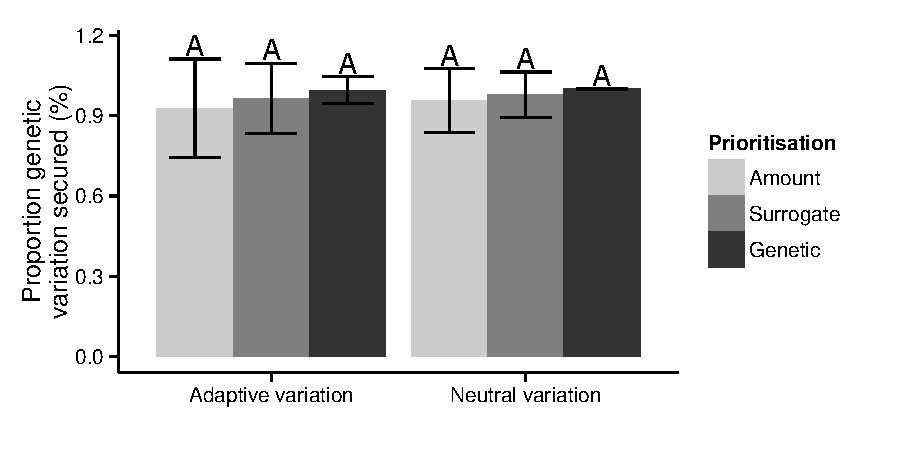
\includegraphics{article_files/figure-latex/unnamed-chunk-2-1.pdf}
\caption{Summary of single species prioritisations. Single species
prioritisations were generated using amount-based targets, amount-based
and surrogate-based targets, and amount-based and genetic-based targets
for each species. Data shows the performance of prioritisations
generated using these three sets of targets. Bars denote means and
standard errors.}
\end{figure}

\subsubsection{Multi-species
prioritisations}\label{multi-species-prioritisations}

\begin{Shaded}
\begin{Highlighting}[]
\CommentTok{# download basemap}
\KeywordTok{data}\NormalTok{(countriesHigh)}
\NormalTok{countries.FPLY <-}\StringTok{ }\NormalTok{countriesHigh[}
    \NormalTok{countriesHigh$ADMIN %in%}\StringTok{ }\KeywordTok{c}\NormalTok{(}
        \StringTok{'Italy'}\NormalTok{, }\StringTok{'Switzerland'}\NormalTok{, }\StringTok{'France'}\NormalTok{, }\StringTok{'Austria'}\NormalTok{,}
        \StringTok{'Germany'}\NormalTok{, }\StringTok{'Slovenia'}\NormalTok{, }\StringTok{'Croatia'}\NormalTok{, }\StringTok{'Hungary'}\NormalTok{,}
        \StringTok{'Monaco'}\NormalTok{, }\StringTok{'Germany'}
    \NormalTok{)}
\NormalTok{,] %>%}\StringTok{ }\NormalTok{spFortify}
\CommentTok{# prepare data for plotting}
\NormalTok{multi.spp.grid.FPLY <-}\StringTok{ }\NormalTok{grid.PLY}
\NormalTok{for (i in }\KeywordTok{seq_along}\NormalTok{(multi.spp.prioritisations))}
    \NormalTok{multi.spp.grid.FPLY@data[[}\KeywordTok{paste0}\NormalTok{(}\StringTok{'v'}\NormalTok{,i)]] <-}\StringTok{ }\KeywordTok{selections}\NormalTok{(multi.spp.prioritisations[[i]])}
\NormalTok{multi.spp.grid.FPLY <-}\StringTok{ }\KeywordTok{spFortify}\NormalTok{(multi.spp.grid.FPLY)}
\CommentTok{# make maps}
\KeywordTok{do.call}\NormalTok{(}
    \NormalTok{grid.arrange,}
    \KeywordTok{append}\NormalTok{(}
        \KeywordTok{llply}\NormalTok{(}
            \KeywordTok{seq_along}\NormalTok{(multi.spp.prioritisations),}
            \NormalTok{function(i) \{}
                \KeywordTok{ggplot}\NormalTok{() +}
\StringTok{                    }\KeywordTok{geom_polygon}\NormalTok{(}\DataTypeTok{data=}\NormalTok{countries.FPLY, }\KeywordTok{aes}\NormalTok{(}\DataTypeTok{x=}\NormalTok{long, }\DataTypeTok{y=}\NormalTok{lat, }\DataTypeTok{group=}\NormalTok{group),}
                        \DataTypeTok{fill=}\StringTok{'grey20'}\NormalTok{, }\DataTypeTok{color=}\StringTok{'grey80'}\NormalTok{) +}
\StringTok{                    }\KeywordTok{geom_polygon}\NormalTok{(}\DataTypeTok{data=}\NormalTok{multi.spp.grid.FPLY, }\KeywordTok{aes_string}\NormalTok{(}\DataTypeTok{x=}\StringTok{'long'}\NormalTok{, }\DataTypeTok{y=}\StringTok{'lat'}\NormalTok{, }
                        \DataTypeTok{group=}\StringTok{'group'}\NormalTok{, }\DataTypeTok{fill=}\KeywordTok{paste0}\NormalTok{(}\StringTok{'v'}\NormalTok{,i)),}
                        \DataTypeTok{alpha=}\FloatTok{0.8}\NormalTok{, }\DataTypeTok{color=}\StringTok{'grey10'}\NormalTok{) +}
\StringTok{                    }\KeywordTok{guides}\NormalTok{(}\DataTypeTok{fill=}\KeywordTok{guide_legend}\NormalTok{(}\DataTypeTok{title=}\StringTok{' '}\NormalTok{)) +}
\StringTok{                    }\KeywordTok{theme_classic}\NormalTok{() +}
\StringTok{                    }\KeywordTok{theme}\NormalTok{(}\DataTypeTok{axis.ticks=}\KeywordTok{element_blank}\NormalTok{(), }\DataTypeTok{axis.text=}\KeywordTok{element_blank}\NormalTok{(),}
                        \DataTypeTok{plot.margin=}\KeywordTok{unit}\NormalTok{(}\KeywordTok{c}\NormalTok{(}\DecValTok{0}\NormalTok{,}\DecValTok{0}\NormalTok{,}\DecValTok{0}\NormalTok{,}\DecValTok{0}\NormalTok{),}\StringTok{'cm'}\NormalTok{), }\DataTypeTok{axis.line=}\KeywordTok{element_blank}\NormalTok{(),}
                        \DataTypeTok{legend.position=}\StringTok{'none'}\NormalTok{) +}
\StringTok{                    }\KeywordTok{coord_cartesian}\NormalTok{(}
                        \DataTypeTok{xlim=}\KeywordTok{buffered.range}\NormalTok{(multi.spp.grid.FPLY$long, }\FloatTok{0.05}\NormalTok{),}
                        \DataTypeTok{ylim=}\KeywordTok{buffered.range}\NormalTok{(multi.spp.grid.FPLY$lat, }\FloatTok{0.05}\NormalTok{)}
                    \NormalTok{) +}
\StringTok{                    }\KeywordTok{xlab}\NormalTok{(}\StringTok{''}\NormalTok{) +}
\StringTok{                    }\KeywordTok{ylab}\NormalTok{(}\StringTok{''}\NormalTok{) +}
\StringTok{                    }\KeywordTok{annotate}\NormalTok{(}\StringTok{'text'}\NormalTok{,}
                        \DataTypeTok{x=}\KeywordTok{min}\NormalTok{(multi.spp.grid.FPLY$long)+}\KeywordTok{diff}\NormalTok{(}\KeywordTok{range}\NormalTok{(multi.spp.grid.FPLY$long)*}\FloatTok{0.1}\NormalTok{),}
                        \DataTypeTok{y=}\KeywordTok{min}\NormalTok{(multi.spp.grid.FPLY$lat)+}\KeywordTok{diff}\NormalTok{(}\KeywordTok{range}\NormalTok{(multi.spp.grid.FPLY$lat)*}\FloatTok{1.01}\NormalTok{),}
                        \DataTypeTok{label=}\NormalTok{letters[i], }\DataTypeTok{hjust=}\DecValTok{1}\NormalTok{, }\DataTypeTok{vjust=}\DecValTok{1}\NormalTok{, }\DataTypeTok{color=}\StringTok{'white'}\NormalTok{, }\DataTypeTok{size=}\DecValTok{8}\NormalTok{)}
            \NormalTok{\}}
        \NormalTok{),}
        \KeywordTok{list}\NormalTok{(}\DataTypeTok{nrow=}\DecValTok{1}\NormalTok{)}
    \NormalTok{)}
\NormalTok{)}
\end{Highlighting}
\end{Shaded}

\begin{figure}[htbp]
\centering
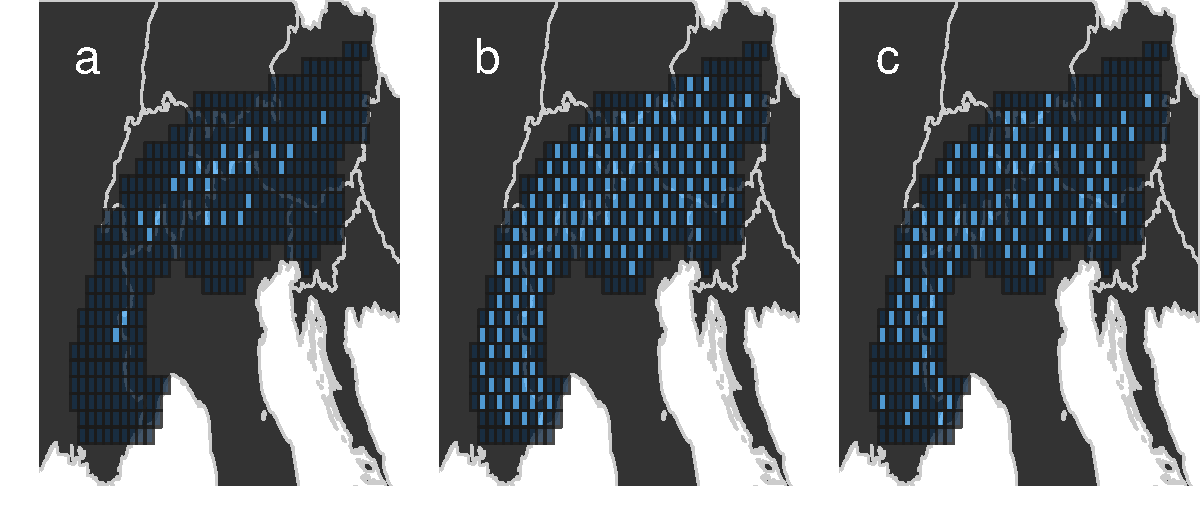
\includegraphics{article_files/figure-latex/unnamed-chunk-3-1.pdf}
\caption{Multi-species prioritisations. Panel (a) shows the
prioritisation generated for using just amount-based targets. Panel (b)
shows the prioritisation generated using amount-based and surrogate
based targets. Panel (c) shows the prioritisation generated using
amount-based and genetic-based targets}
\end{figure}

\begin{Shaded}
\begin{Highlighting}[]
\CommentTok{# prepare data for plotting}
\NormalTok{multi.spp.PDF <-}\StringTok{ }\KeywordTok{expand.grid}\NormalTok{(}
    \DataTypeTok{Prioritisation=}\KeywordTok{unique}\NormalTok{(multi.spp.SDF$Prioritisation),}
    \DataTypeTok{Metric=}\KeywordTok{unique}\NormalTok{(multi.spp.SDF$Metric))}
\NormalTok{multi.spp.PDF <-}\StringTok{ }\KeywordTok{cbind}\NormalTok{(multi.spp.PDF,}
    \KeywordTok{as.data.frame}\NormalTok{(}\KeywordTok{predict}\NormalTok{(multi.spp.GLM, multi.spp.PDF,}
        \DataTypeTok{type=}\StringTok{'response'}\NormalTok{, }\DataTypeTok{se.fit=}\OtherTok{TRUE}\NormalTok{))) %>%}
\StringTok{    }\KeywordTok{mutate}\NormalTok{(}\DataTypeTok{lower=}\NormalTok{fit-se.fit, }\DataTypeTok{upper=}\NormalTok{fit+se.fit,}
        \DataTypeTok{letters=}\KeywordTok{toupper}\NormalTok{(}\KeywordTok{cld}\NormalTok{(multi.spp.MCP)$mcletters$Letters),}
        \DataTypeTok{letter_pos=}\NormalTok{upper}\FloatTok{+0.05}\NormalTok{)}
\CommentTok{# make plot}
\KeywordTok{ggplot}\NormalTok{(}\KeywordTok{aes}\NormalTok{(}\DataTypeTok{x=}\NormalTok{Metric,}\DataTypeTok{y=}\NormalTok{fit,}\DataTypeTok{fill=}\NormalTok{Prioritisation),}
    \DataTypeTok{data=}\NormalTok{multi.spp.PDF) +}
\StringTok{    }\KeywordTok{geom_bar}\NormalTok{(}\DataTypeTok{position=}\KeywordTok{position_dodge}\NormalTok{(}\FloatTok{0.9}\NormalTok{),}
        \DataTypeTok{stat=}\StringTok{'identity'}\NormalTok{) +}
\StringTok{    }\KeywordTok{geom_errorbar}\NormalTok{(}
        \KeywordTok{aes}\NormalTok{(}\DataTypeTok{ymin=}\NormalTok{lower,}\DataTypeTok{ymax=}\NormalTok{upper),}
        \DataTypeTok{position=}\KeywordTok{position_dodge}\NormalTok{(}\FloatTok{0.9}\NormalTok{), }\DataTypeTok{width=}\FloatTok{0.6}\NormalTok{) +}
\StringTok{    }\KeywordTok{geom_text}\NormalTok{(}\KeywordTok{aes}\NormalTok{(}\DataTypeTok{x=}\NormalTok{Metric, }\DataTypeTok{y=}\NormalTok{letter_pos,}
        \DataTypeTok{label=}\NormalTok{letters), }\DataTypeTok{position=}\KeywordTok{position_dodge}\NormalTok{(}\FloatTok{0.9}\NormalTok{)) +}
\StringTok{    }\KeywordTok{scale_fill_manual}\NormalTok{(}\DataTypeTok{name=}\StringTok{'Prioritisation'}\NormalTok{,}
        \DataTypeTok{values=}\KeywordTok{c}\NormalTok{(}\StringTok{'grey80'}\NormalTok{,}\StringTok{'grey50'}\NormalTok{,}\StringTok{'grey20'}\NormalTok{)) +}
\StringTok{    }\KeywordTok{ylab}\NormalTok{(}\StringTok{'Proportion genetic}\CharTok{\textbackslash{}n}\StringTok{variation secured (%)'}\NormalTok{) +}
\StringTok{    }\KeywordTok{xlab}\NormalTok{(}\StringTok{''}\NormalTok{) +}
\StringTok{    }\KeywordTok{theme_classic}\NormalTok{()}
\end{Highlighting}
\end{Shaded}

\begin{verbatim}
## ymax not defined: adjusting position using y instead
\end{verbatim}

\begin{figure}[htbp]
\centering
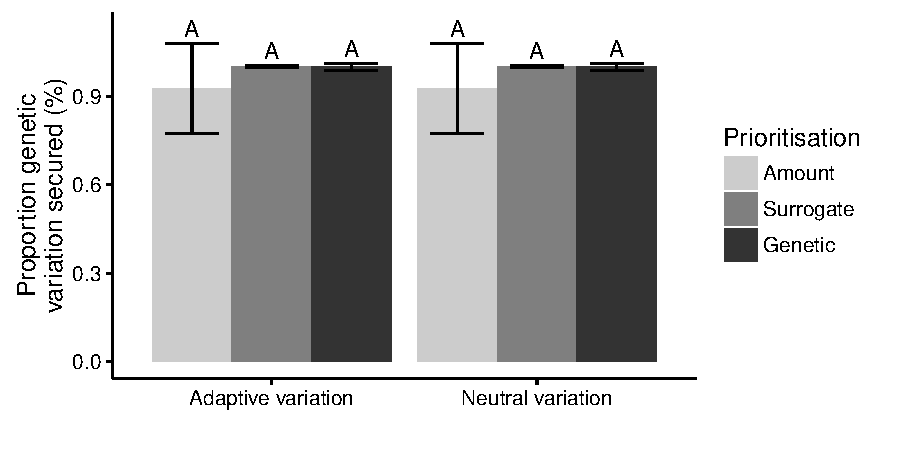
\includegraphics{article_files/figure-latex/unnamed-chunk-4-1.pdf}
\caption{Summary of multi-species prioritisations. Three prioritisations
were generated using amount-based targets, amount-based and
surrogate-based targets, and amount-based and genetic-based targets for
each species. Data shows the performance of these prioritisations based
on how much genetic variation they explain. Bars denote means and
standard errors.}
\end{figure}

\subsubsection{Pareo-frontier analysis}\label{pareo-frontier-analysis}

\begin{Shaded}
\begin{Highlighting}[]
\CommentTok{# make plots}
\NormalTok{p1 <-}\StringTok{ }\KeywordTok{ggplot}\NormalTok{(}\DataTypeTok{data=}\NormalTok{env.pareto.DF) +}
\StringTok{    }\KeywordTok{geom_line}\NormalTok{(}\KeywordTok{aes}\NormalTok{(}\DataTypeTok{x=}\NormalTok{Surrogate.target,}\DataTypeTok{y=}\NormalTok{adaptive.held,}\DataTypeTok{group=}\NormalTok{Species),}
        \DataTypeTok{alpha=}\FloatTok{0.5}\NormalTok{) +}
\StringTok{    }\KeywordTok{xlab}\NormalTok{(}\StringTok{'Environmental variation secured (%)'}\NormalTok{) +}
\StringTok{    }\KeywordTok{ylab}\NormalTok{(}\StringTok{'Adaptive genetic}\CharTok{\textbackslash{}n}\StringTok{variation secured (%)'}\NormalTok{) +}
\StringTok{    }\KeywordTok{theme_classic}\NormalTok{()}
\NormalTok{p2 <-}\StringTok{ }\KeywordTok{ggplot}\NormalTok{(}\DataTypeTok{data=}\NormalTok{geo.pareto.DF) +}
\StringTok{    }\KeywordTok{geom_line}\NormalTok{(}\KeywordTok{aes}\NormalTok{(}\DataTypeTok{x=}\NormalTok{Surrogate.target,}\DataTypeTok{y=}\NormalTok{neutral.held,}\DataTypeTok{group=}\NormalTok{Species),}
        \DataTypeTok{alpha=}\FloatTok{0.5}\NormalTok{) +}
\StringTok{    }\KeywordTok{xlab}\NormalTok{(}\StringTok{'Geographic variation secured (%)'}\NormalTok{) +}
\StringTok{    }\KeywordTok{ylab}\NormalTok{(}\StringTok{'Neutral genetic}\CharTok{\textbackslash{}n}\StringTok{variation secured (%)'}\NormalTok{) +}
\StringTok{    }\KeywordTok{theme_classic}\NormalTok{()}
\KeywordTok{grid.arrange}\NormalTok{(p1, p2, }\DataTypeTok{nrow=}\DecValTok{1}\NormalTok{)}
\end{Highlighting}
\end{Shaded}

\begin{figure}[htbp]
\centering
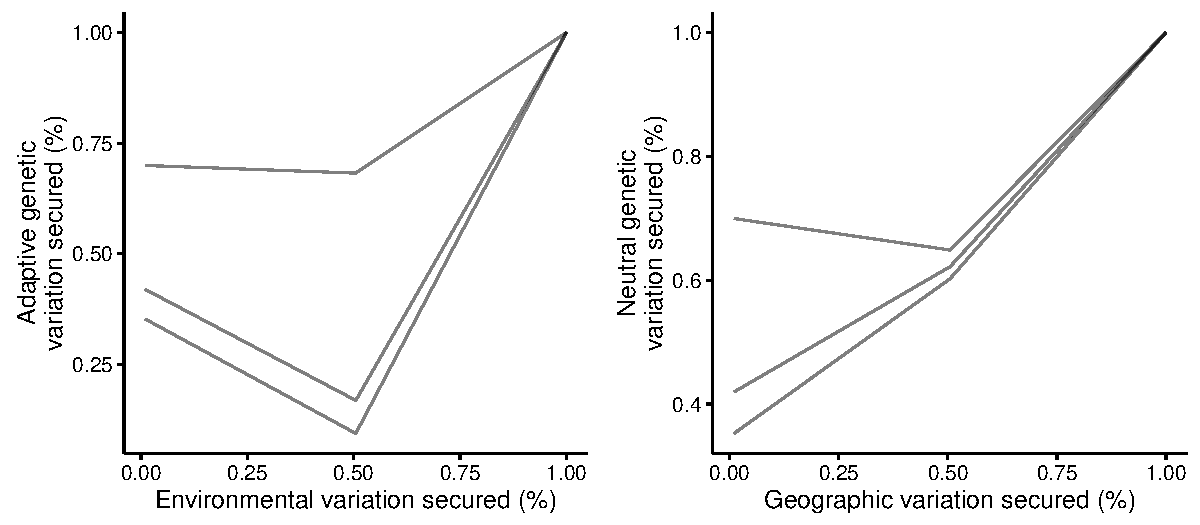
\includegraphics{article_files/figure-latex/unnamed-chunk-5-1.pdf}
\caption{The relationship between surrogates and genetic variation
secured in prioritisations.}
\end{figure}

\subsection{Discussion}\label{discussion}

\subsection{Acknowledgements}\label{acknowledgements}

JOH is funded by an Australian Postgraduate Award (APA) scholarship. RAF
has an Australian Research Council Future Fellowship. This work was
supported by the Centre of Excellence for Environmental Decisions (CEED)
and the Landscape Ecology and Conservation Group (LEC) at The University
of Queensland.

\subsection{References}\label{references}

\subsection{Figures}\label{figures}

\subsection{Tables}\label{tables}

\subsection{Supporting Information}\label{supporting-information}

\subsubsection{Figure S1: Species
distributions}\label{figure-s1-species-distributions}

\begin{Shaded}
\begin{Highlighting}[]
\NormalTok{## plot map of species distributions}
\CommentTok{# fortify data}
\NormalTok{grid.FPLY <-}\StringTok{ }\KeywordTok{spFortify}\NormalTok{(grid.PLY)}
\NormalTok{spp.grid.FPLY <-}\StringTok{ }\KeywordTok{ldply}\NormalTok{(}\KeywordTok{unique}\NormalTok{(spp.samples.DF$species), function(x) \{}
        \NormalTok{z <-}\StringTok{ }\NormalTok{grid.FPLY[,}\KeywordTok{c}\NormalTok{(}\StringTok{'long'}\NormalTok{, }\StringTok{'lat'}\NormalTok{, }\StringTok{'group'}\NormalTok{, x),drop=}\OtherTok{FALSE}\NormalTok{]}
        \KeywordTok{names}\NormalTok{(z)[}\DecValTok{4}\NormalTok{] <-}\StringTok{ 'presence'}
        \NormalTok{z$species <-}\StringTok{ }\KeywordTok{gsub}\NormalTok{(}\StringTok{'}\CharTok{\textbackslash{}\textbackslash{}}\StringTok{_'}\NormalTok{, }\StringTok{' '}\NormalTok{, x)}
        \KeywordTok{return}\NormalTok{(z)}
    \NormalTok{\}}
\NormalTok{)}
\CommentTok{# plot species data}
\KeywordTok{ggplot}\NormalTok{() +}
\StringTok{    }\KeywordTok{geom_polygon}\NormalTok{(}\DataTypeTok{data=}\NormalTok{countries.FPLY, }\KeywordTok{aes}\NormalTok{(}\DataTypeTok{x=}\NormalTok{long, }\DataTypeTok{y=}\NormalTok{lat, }\DataTypeTok{group=}\NormalTok{group),}
        \DataTypeTok{fill=}\StringTok{'grey20'}\NormalTok{, }\DataTypeTok{color=}\StringTok{'grey80'}\NormalTok{) +}
\StringTok{    }\KeywordTok{geom_polygon}\NormalTok{(}\DataTypeTok{data=}\NormalTok{spp.grid.FPLY, }\KeywordTok{aes}\NormalTok{(}\DataTypeTok{x=}\NormalTok{long, }\DataTypeTok{y=}\NormalTok{lat, }
        \DataTypeTok{group=}\NormalTok{group, }\DataTypeTok{fill=}\NormalTok{presence), }\DataTypeTok{alpha=}\FloatTok{0.8}\NormalTok{, }\DataTypeTok{color=}\StringTok{'grey10'}\NormalTok{) +}
\StringTok{    }\KeywordTok{theme_classic}\NormalTok{() +}
\StringTok{    }\KeywordTok{guides}\NormalTok{(}\DataTypeTok{fill=}\KeywordTok{guide_legend}\NormalTok{(}\DataTypeTok{title=}\StringTok{'Presence'}\NormalTok{)) +}
\StringTok{    }\KeywordTok{theme}\NormalTok{(}\DataTypeTok{axis.ticks=}\KeywordTok{element_blank}\NormalTok{(), }\DataTypeTok{axis.text=}\KeywordTok{element_blank}\NormalTok{(),}
        \DataTypeTok{axis.line=}\KeywordTok{element_blank}\NormalTok{()) +}
\StringTok{    }\KeywordTok{coord_cartesian}\NormalTok{(}
        \DataTypeTok{xlim=}\KeywordTok{buffered.range}\NormalTok{(grid.FPLY$long, }\FloatTok{0.05}\NormalTok{),}
        \DataTypeTok{ylim=}\KeywordTok{buffered.range}\NormalTok{(grid.FPLY$lat, }\FloatTok{0.05}\NormalTok{)}
    \NormalTok{) +}
\StringTok{    }\KeywordTok{xlab}\NormalTok{(}\StringTok{''}\NormalTok{) +}
\StringTok{    }\KeywordTok{ylab}\NormalTok{(}\StringTok{''}\NormalTok{) +}
\StringTok{    }\KeywordTok{facet_wrap}\NormalTok{(~}\StringTok{ }\NormalTok{species, }\DataTypeTok{ncol=}\DecValTok{4}\NormalTok{)}
\end{Highlighting}
\end{Shaded}

\begin{figure}
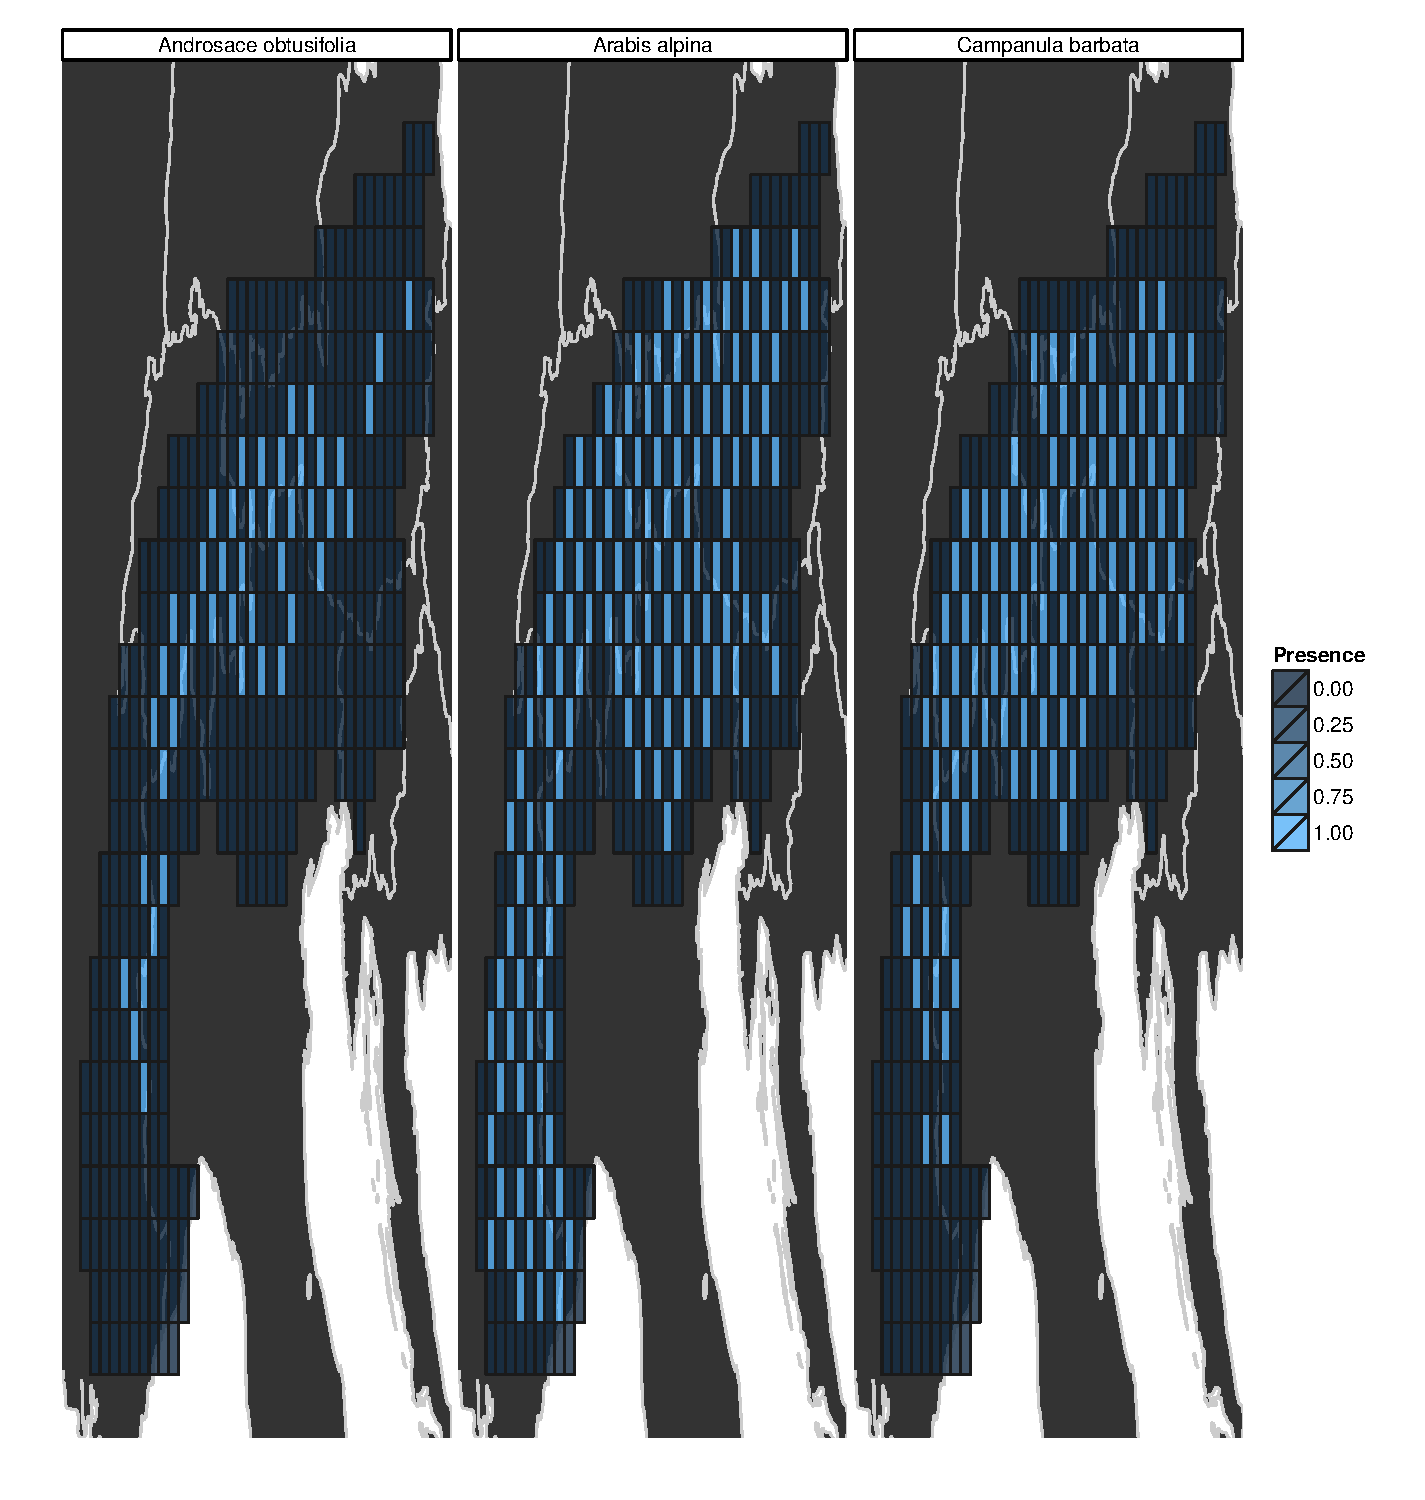
\includegraphics[width=7.5in,height=8.5in]{article_files/figure-latex/unnamed-chunk-6-1} \caption{Species distributions. Squares represent planning units. For a given species, planning units that were found to be inhabited are denoted with bright blue.}\label{fig:unnamed-chunk-6}
\end{figure}

\begin{Shaded}
\begin{Highlighting}[]
\CommentTok{# calculate species richness}
\NormalTok{grid.PLY$Species_richness <-}\StringTok{ }\NormalTok{grid.PLY@data %>%}
\StringTok{    }\KeywordTok{select}\NormalTok{(}\DecValTok{5}\NormalTok{:(}\DecValTok{4}\NormalTok{+n.spp)) %>%}\StringTok{ }\KeywordTok{as.matrix}\NormalTok{() %>%}\StringTok{ }\KeywordTok{rowSums}\NormalTok{()}

\CommentTok{# plot species richness}
\KeywordTok{ggplot}\NormalTok{() +}
\StringTok{    }\KeywordTok{geom_polygon}\NormalTok{(}\DataTypeTok{data=}\NormalTok{countries.FPLY, }\KeywordTok{aes}\NormalTok{(}\DataTypeTok{x=}\NormalTok{long, }\DataTypeTok{y=}\NormalTok{lat, }\DataTypeTok{group=}\NormalTok{group),}
        \DataTypeTok{fill=}\StringTok{'grey20'}\NormalTok{, }\DataTypeTok{color=}\StringTok{'grey80'}\NormalTok{) +}
\StringTok{    }\KeywordTok{geom_polygon}\NormalTok{(}\DataTypeTok{data=}\KeywordTok{spFortify}\NormalTok{(grid.PLY), }\KeywordTok{aes}\NormalTok{(}\DataTypeTok{x=}\NormalTok{long, }\DataTypeTok{y=}\NormalTok{lat, }
        \DataTypeTok{group=}\NormalTok{group, }\DataTypeTok{fill=}\NormalTok{Species_richness), }\DataTypeTok{alpha=}\FloatTok{0.8}\NormalTok{, }\DataTypeTok{color=}\StringTok{'grey10'}\NormalTok{) +}
\StringTok{    }\KeywordTok{guides}\NormalTok{(}\DataTypeTok{fill=}\KeywordTok{guide_legend}\NormalTok{(}\DataTypeTok{title=}\StringTok{'Count (#)'}\NormalTok{)) +}
\StringTok{    }\KeywordTok{theme_classic}\NormalTok{() +}
\StringTok{    }\KeywordTok{theme}\NormalTok{(}\DataTypeTok{axis.ticks=}\KeywordTok{element_blank}\NormalTok{(), }\DataTypeTok{axis.text=}\KeywordTok{element_blank}\NormalTok{(),}
        \DataTypeTok{axis.line=}\KeywordTok{element_blank}\NormalTok{()) +}
\StringTok{    }\KeywordTok{coord_cartesian}\NormalTok{(}
        \DataTypeTok{xlim=}\KeywordTok{buffered.range}\NormalTok{(grid.FPLY$long, }\FloatTok{0.05}\NormalTok{),}
        \DataTypeTok{ylim=}\KeywordTok{buffered.range}\NormalTok{(grid.FPLY$lat, }\FloatTok{0.05}\NormalTok{)}
    \NormalTok{) +}
\StringTok{    }\KeywordTok{xlab}\NormalTok{(}\StringTok{''}\NormalTok{) +}
\StringTok{    }\KeywordTok{ylab}\NormalTok{(}\StringTok{''}\NormalTok{) +}
\StringTok{    }\KeywordTok{ggtitle}\NormalTok{(}\StringTok{'Species richness'}\NormalTok{)}
\end{Highlighting}
\end{Shaded}

\begin{figure}[htbp]
\centering
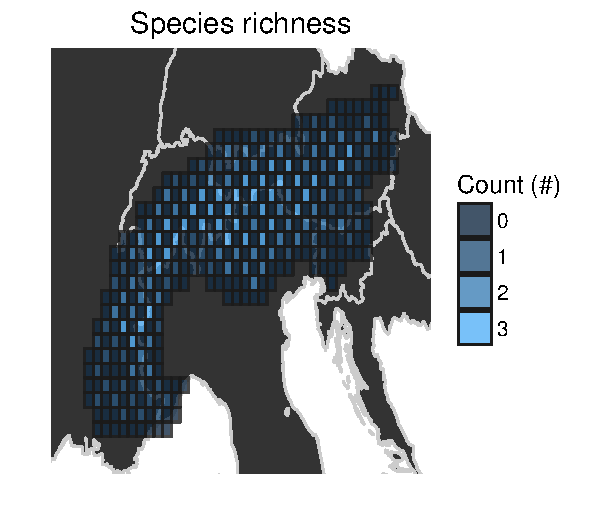
\includegraphics{article_files/figure-latex/unnamed-chunk-7-1.pdf}
\caption{Species richness. Squares denote planning units. Planning units
with a brighter color are inhabited by more species.}
\end{figure}

\subsubsection{Figure S2: Maps of climatic
variation}\label{figure-s2-maps-of-climatic-variation}

\begin{Shaded}
\begin{Highlighting}[]
\KeywordTok{do.call}\NormalTok{(}
    \NormalTok{grid.arrange,}
        \KeywordTok{append}\NormalTok{(}
        \KeywordTok{llply}\NormalTok{(}\KeywordTok{grep}\NormalTok{(}\StringTok{'^env}\CharTok{\textbackslash{}\textbackslash{}}\StringTok{_.*$'}\NormalTok{, }\KeywordTok{names}\NormalTok{(grid.DF), }\DataTypeTok{value=}\OtherTok{TRUE}\NormalTok{), function(x) \{}
            \KeywordTok{ggplot}\NormalTok{() +}
\StringTok{                }\KeywordTok{geom_polygon}\NormalTok{(}\DataTypeTok{data=}\NormalTok{countries.FPLY, }\KeywordTok{aes}\NormalTok{(}\DataTypeTok{x=}\NormalTok{long, }\DataTypeTok{y=}\NormalTok{lat, }\DataTypeTok{group=}\NormalTok{group),}
                    \DataTypeTok{fill=}\StringTok{'grey20'}\NormalTok{, }\DataTypeTok{color=}\StringTok{'grey80'}\NormalTok{) +}
\StringTok{                }\KeywordTok{geom_polygon}\NormalTok{(}\DataTypeTok{data=}\NormalTok{grid.FPLY, }\KeywordTok{aes_string}\NormalTok{(}\DataTypeTok{x=}\StringTok{'long'}\NormalTok{, }\DataTypeTok{y=}\StringTok{'lat'}\NormalTok{, }
                    \DataTypeTok{group=}\StringTok{'group'}\NormalTok{, }\DataTypeTok{fill=}\NormalTok{x),}
                    \DataTypeTok{alpha=}\FloatTok{0.8}\NormalTok{, }\DataTypeTok{color=}\StringTok{'grey10'}\NormalTok{) +}
\StringTok{                }\KeywordTok{guides}\NormalTok{(}\DataTypeTok{fill=}\KeywordTok{guide_legend}\NormalTok{(}\DataTypeTok{title=}\StringTok{' '}\NormalTok{)) +}
\StringTok{                }\KeywordTok{theme_classic}\NormalTok{() +}
\StringTok{                }\KeywordTok{theme}\NormalTok{(}\DataTypeTok{axis.ticks=}\KeywordTok{element_blank}\NormalTok{(), }\DataTypeTok{axis.text=}\KeywordTok{element_blank}\NormalTok{(),}
                    \DataTypeTok{plot.margin=}\KeywordTok{unit}\NormalTok{(}\KeywordTok{c}\NormalTok{(}\DecValTok{0}\NormalTok{,}\DecValTok{0}\NormalTok{,}\DecValTok{0}\NormalTok{,}\DecValTok{0}\NormalTok{),}\StringTok{'cm'}\NormalTok{), }\DataTypeTok{axis.line=}\KeywordTok{element_blank}\NormalTok{()) +}
\StringTok{                }\KeywordTok{coord_cartesian}\NormalTok{(}
                    \DataTypeTok{xlim=}\KeywordTok{buffered.range}\NormalTok{(grid.FPLY$long, }\FloatTok{0.05}\NormalTok{),}
                    \DataTypeTok{ylim=}\KeywordTok{buffered.range}\NormalTok{(grid.FPLY$lat, }\FloatTok{0.05}\NormalTok{)}
                \NormalTok{) +}
\StringTok{                }\KeywordTok{xlab}\NormalTok{(}\StringTok{''}\NormalTok{) +}
\StringTok{                }\KeywordTok{ylab}\NormalTok{(}\StringTok{''}\NormalTok{) +}
\StringTok{                }\KeywordTok{ggtitle}\NormalTok{(}\KeywordTok{paste0}\NormalTok{(}\StringTok{'PC '}\NormalTok{, }\KeywordTok{substr}\NormalTok{(x, }\KeywordTok{nchar}\NormalTok{(x), }\KeywordTok{nchar}\NormalTok{(x))))}
        \NormalTok{\}),}
        \KeywordTok{list}\NormalTok{(}\DataTypeTok{ncol=}\DecValTok{2}\NormalTok{)}
    \NormalTok{)}
\NormalTok{)}
\end{Highlighting}
\end{Shaded}

\begin{figure}[htbp]
\centering
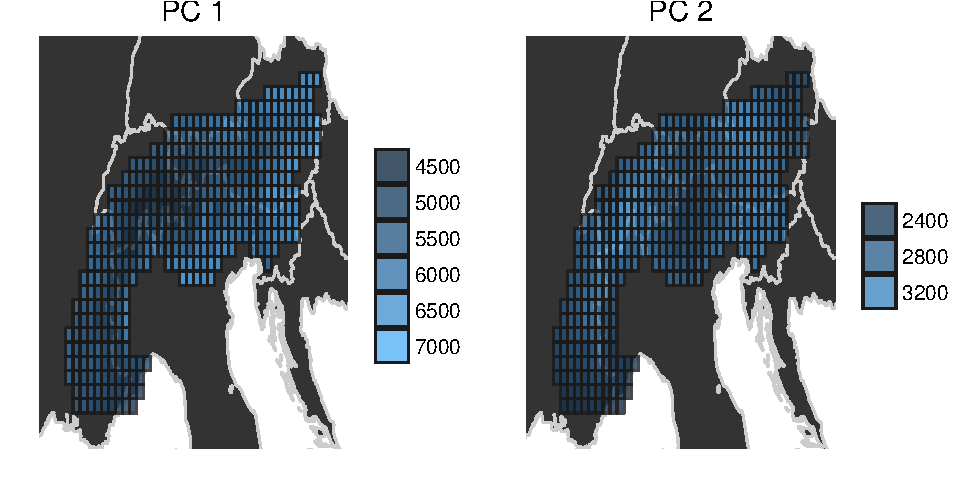
\includegraphics{article_files/figure-latex/unnamed-chunk-8-1.pdf}
\caption{Climatic variation. Each panel depicts variation based on a
different principle component (PC). Sqaures represent planning units.
The color of each planning unit denotes the average priciniple component
value of pixels inside it. Planning units with more similar colors have
more similar climates regimes.}
\end{figure}

\subsubsection{Figure S3. Number populations in each
species.}\label{figure-s3.-number-populations-in-each-species.}

\subsubsection{Figure S4. Distribution of populations for each
species.}\label{figure-s4.-distribution-of-populations-for-each-species.}

\begin{Shaded}
\begin{Highlighting}[]
\NormalTok{plot.spp.mds <-}\StringTok{ }\NormalTok{function(i) \{}
    \CommentTok{# define function}
    \NormalTok{make.mds.plot <-}\StringTok{ }\NormalTok{function(j,k) \{}
        \KeywordTok{ggplot}\NormalTok{() +}
\StringTok{            }\KeywordTok{geom_polygon}\NormalTok{(}\DataTypeTok{data=}\NormalTok{countries.FPLY, }\KeywordTok{aes}\NormalTok{(}\DataTypeTok{x=}\NormalTok{long, }\DataTypeTok{y=}\NormalTok{lat, }\DataTypeTok{group=}\NormalTok{group),}
                \DataTypeTok{fill=}\StringTok{'grey20'}\NormalTok{, }\DataTypeTok{color=}\StringTok{'grey80'}\NormalTok{) +}
\StringTok{            }\KeywordTok{geom_polygon}\NormalTok{(}\DataTypeTok{data=}\NormalTok{grid.FPLY, }\KeywordTok{aes_string}\NormalTok{(}\DataTypeTok{x=}\StringTok{'long'}\NormalTok{, }\DataTypeTok{y=}\StringTok{'lat'}\NormalTok{, }
                \DataTypeTok{group=}\StringTok{'group'}\NormalTok{, }\DataTypeTok{fill=}\KeywordTok{paste0}\NormalTok{(}\KeywordTok{unique}\NormalTok{(spp.samples.DF$species)[i], }\StringTok{'_'}\NormalTok{, j, }\StringTok{'_d'}\NormalTok{,k)),}
                \DataTypeTok{alpha=}\FloatTok{0.8}\NormalTok{, }\DataTypeTok{color=}\StringTok{'grey10'}\NormalTok{) +}
\StringTok{            }\KeywordTok{guides}\NormalTok{(}\DataTypeTok{fill=}\KeywordTok{guide_legend}\NormalTok{(}\DataTypeTok{title=}\StringTok{' '}\NormalTok{)) +}
\StringTok{            }\KeywordTok{theme_classic}\NormalTok{() +}
\StringTok{            }\KeywordTok{theme}\NormalTok{(}\DataTypeTok{axis.ticks=}\KeywordTok{element_blank}\NormalTok{(), }\DataTypeTok{axis.text=}\KeywordTok{element_blank}\NormalTok{(),}
                \DataTypeTok{plot.margin=}\KeywordTok{unit}\NormalTok{(}\KeywordTok{c}\NormalTok{(}\DecValTok{0}\NormalTok{,}\DecValTok{0}\NormalTok{,}\DecValTok{0}\NormalTok{,}\DecValTok{0}\NormalTok{),}\StringTok{'cm'}\NormalTok{), }\DataTypeTok{axis.line=}\KeywordTok{element_blank}\NormalTok{()) +}
\StringTok{            }\KeywordTok{coord_cartesian}\NormalTok{(}
                \DataTypeTok{xlim=}\KeywordTok{buffered.range}\NormalTok{(grid.FPLY$long, }\FloatTok{0.05}\NormalTok{),}
                \DataTypeTok{ylim=}\KeywordTok{buffered.range}\NormalTok{(grid.FPLY$lat, }\FloatTok{0.05}\NormalTok{)}
            \NormalTok{) +}
\StringTok{            }\KeywordTok{xlab}\NormalTok{(}\StringTok{''}\NormalTok{) +}
\StringTok{            }\KeywordTok{ylab}\NormalTok{(}\StringTok{''}\NormalTok{) +}
\StringTok{            }\KeywordTok{ggtitle}\NormalTok{(}\KeywordTok{paste0}\NormalTok{(j,}\StringTok{' ('}\NormalTok{,k,}\StringTok{')'}\NormalTok{))}
    \NormalTok{\}}
    \CommentTok{# init}
    \NormalTok{adapt.col <-}\StringTok{ }\KeywordTok{paste0}\NormalTok{(}\KeywordTok{unique}\NormalTok{(spp.samples.DF$species)[i], }\StringTok{'_adaptive_d1'}\NormalTok{)}
    \NormalTok{neutral.col <-}\StringTok{ }\KeywordTok{paste0}\NormalTok{(}\KeywordTok{unique}\NormalTok{(spp.samples.DF$species)[i], }\StringTok{'_neutral_d1'}\NormalTok{)}
    \NormalTok{plotLST <-}\StringTok{ }\KeywordTok{list}\NormalTok{()}
    \CommentTok{# make adaptive plot}
    \NormalTok{if (adapt.col %in%}\StringTok{ }\KeywordTok{names}\NormalTok{(grid.FPLY)) \{}
        \NormalTok{for (k in }\KeywordTok{seq_len}\NormalTok{(mds.k))}
            \NormalTok{plotLST <-}\StringTok{ }\KeywordTok{append}\NormalTok{(plotLST, }\KeywordTok{list}\NormalTok{(}\KeywordTok{make.mds.plot}\NormalTok{(}\StringTok{'adaptive'}\NormalTok{, k)))}
    \NormalTok{\} }
    \CommentTok{# make neutral plot}
    \NormalTok{if (neutral.col %in%}\StringTok{ }\KeywordTok{names}\NormalTok{(grid.FPLY)) \{}
        \NormalTok{for (k in }\KeywordTok{seq_len}\NormalTok{(mds.k))}
            \NormalTok{plotLST <-}\StringTok{ }\KeywordTok{append}\NormalTok{(plotLST, }\KeywordTok{list}\NormalTok{(}\KeywordTok{make.mds.plot}\NormalTok{(}\StringTok{'neutral'}\NormalTok{, k)))}
    \NormalTok{\} }
    \CommentTok{# make plot}
    \KeywordTok{do.call}\NormalTok{(}
        \NormalTok{grid.arrange,}
        \KeywordTok{append}\NormalTok{(}
            \NormalTok{plotLST,}
            \KeywordTok{list}\NormalTok{(}\DataTypeTok{ncol=}\DecValTok{6}\NormalTok{)}
        \NormalTok{)}
    \NormalTok{)}
\NormalTok{\}}
\end{Highlighting}
\end{Shaded}

\subsubsection{Figures S}\label{figures-s}

\begin{Shaded}
\begin{Highlighting}[]
\KeywordTok{plot.spp.mds}\NormalTok{(}\DecValTok{1}\NormalTok{)}
\end{Highlighting}
\end{Shaded}

\begin{figure}[htbp]
\centering
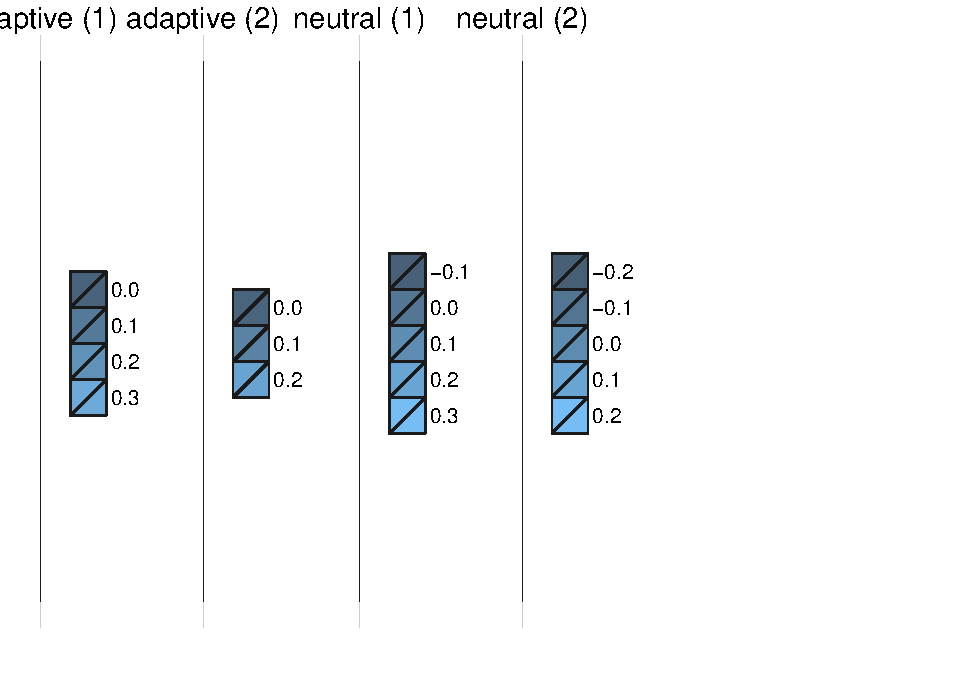
\includegraphics{article_files/figure-latex/unnamed-chunk-12-1.pdf}
\caption{Distribution of adaptive and neutral genetic variation in
\textit{Androsace obtusifolia}. Each square represents a planning unit.
The color of each planning unit panel corresponds to ordination values.
Planning units with similar colors contain individiduals with similar
genetic variation.}
\end{figure}

\begin{Shaded}
\begin{Highlighting}[]
\KeywordTok{plot.spp.mds}\NormalTok{(}\DecValTok{2}\NormalTok{)}
\end{Highlighting}
\end{Shaded}

\begin{figure}[htbp]
\centering
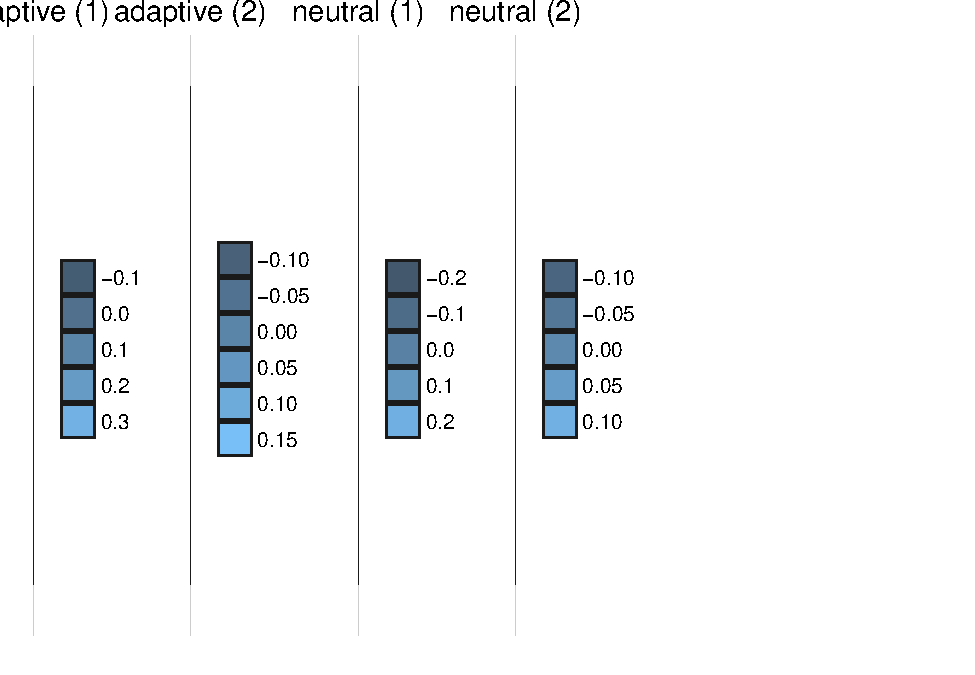
\includegraphics{article_files/figure-latex/unnamed-chunk-13-1.pdf}
\caption{Distribution of adaptive and neutral genetic variation in
\textit{Arabis alpina}. See Figure XX caption for conventions.}
\end{figure}

\begin{Shaded}
\begin{Highlighting}[]
\KeywordTok{plot.spp.mds}\NormalTok{(}\DecValTok{3}\NormalTok{)}
\end{Highlighting}
\end{Shaded}

\begin{figure}[htbp]
\centering
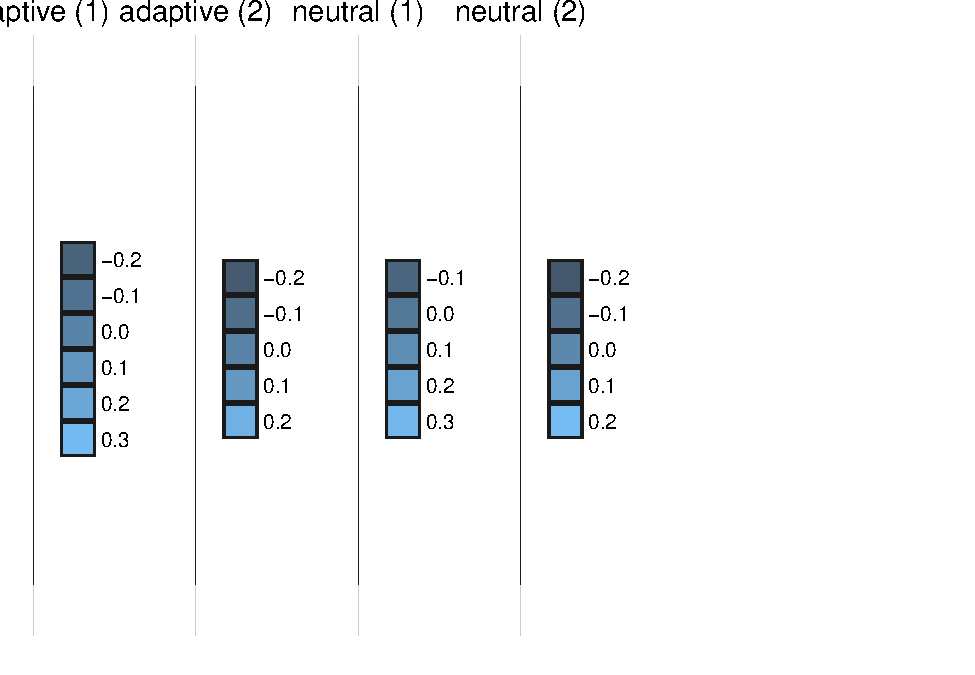
\includegraphics{article_files/figure-latex/unnamed-chunk-14-1.pdf}
\caption{Distribution of adaptive and neutral genetic variation in
\textit{Campanula barbata}. See Figure XX caption for conventions.}
\end{figure}

\subsubsection{Table S1: Principle components analysis on climatic
variation}\label{table-s1-principle-components-analysis-on-climatic-variation}

\begin{Shaded}
\begin{Highlighting}[]
\NormalTok{## make results table showing Eigen values}
\NormalTok{knitr::}\KeywordTok{kable}\NormalTok{(}
    \NormalTok{pca.DF,}
    \DataTypeTok{digits=}\DecValTok{2}\NormalTok{,}
    \DataTypeTok{caption=}\StringTok{'Summary of principle components analysis (PCA) on bioclimatic variation across the study area. The first two principle components (PCs) were used for subsequent analysis.'}\NormalTok{,}
    \DataTypeTok{align=}\KeywordTok{c}\NormalTok{(}\StringTok{'l'}\NormalTok{, }\StringTok{'c'}\NormalTok{, }\StringTok{'c'}\NormalTok{, }\StringTok{'c'}\NormalTok{)}
\NormalTok{)}
\end{Highlighting}
\end{Shaded}

\begin{longtable}[c]{@{}lccc@{}}
\toprule\addlinespace
Principle Component & Eigen Value & Variation explained (\%) &
Accumulative variation explained (\%)
\\\addlinespace
\midrule\endhead
1 & 216765.14 & 82.67 & 82.67
\\\addlinespace
2 & 38177.84 & 14.56 & 97.23
\\\addlinespace
3 & 5356.75 & 2.04 & 99.27
\\\addlinespace
4 & 1216.67 & 0.46 & 99.73
\\\addlinespace
5 & 700.39 & 0.27 & 100.00
\\\addlinespace
\bottomrule
\addlinespace
\caption{Summary of principle components analysis (PCA) on bioclimatic
variation across the study area. The first two principle components
(PCs) were used for subsequent analysis.}
\end{longtable}

\subsubsection{Table S2: BayeScan
Results}\label{table-s2-bayescan-results}

\begin{Shaded}
\begin{Highlighting}[]
\NormalTok{knitr::}\KeywordTok{kable}\NormalTok{(}
    \KeywordTok{format.table}\NormalTok{(}
        \KeywordTok{ldply}\NormalTok{(}
            \KeywordTok{seq_along}\NormalTok{(}\KeywordTok{unique}\NormalTok{(spp.samples.DF$species)), }
            \NormalTok{function(i) \{}
                \KeywordTok{data.frame}\NormalTok{(}
                    \DataTypeTok{Species=}\KeywordTok{paste0}\NormalTok{(}\StringTok{'}\CharTok{\textbackslash{}\textbackslash{}}\StringTok{textit\{'}\NormalTok{,}\KeywordTok{gsub}\NormalTok{(}\StringTok{'}\CharTok{\textbackslash{}\textbackslash{}}\StringTok{_'}\NormalTok{, }\StringTok{' '}\NormalTok{, }\KeywordTok{unique}\NormalTok{(spp.samples.DF$species)[i]),}\StringTok{'\}'}\NormalTok{),}
                    \DataTypeTok{Primer=}\NormalTok{spp.BayeScan.sample.loci.subset.LST[[i]]@data@primers,}
                    \DataTypeTok{Probability=}\NormalTok{spp.BayeScan.sample.loci.subset.LST[[i]]@results@summary[[}\DecValTok{2}\NormalTok{]],}
                    \DataTypeTok{qval=}\NormalTok{spp.BayeScan.sample.loci.subset.LST[[i]]@results@summary[[}\DecValTok{4}\NormalTok{]],}
                    \DataTypeTok{alpha=}\NormalTok{spp.BayeScan.sample.loci.subset.LST[[i]]@results@summary[[}\DecValTok{5}\NormalTok{]],}
                    \DataTypeTok{fst=}\NormalTok{spp.BayeScan.sample.loci.subset.LST[[i]]@results@summary[[}\DecValTok{6}\NormalTok{]],}
                    \DataTypeTok{Type=}\NormalTok{spp.BayeScan.sample.loci.subset.LST[[i]]@results@summary[[}\DecValTok{7}\NormalTok{]]}
                \NormalTok{)}
            \NormalTok{\}}
        \NormalTok{),}
        \DataTypeTok{omit=}\StringTok{'Type'}
    \NormalTok{),}
    \DataTypeTok{digits=}\DecValTok{2}\NormalTok{,}
    \DataTypeTok{col.names=}\KeywordTok{c}\NormalTok{(}\StringTok{'Species'}\NormalTok{, }\StringTok{'Primer'}\NormalTok{, }\StringTok{'Probability'}\NormalTok{, }\StringTok{'q-value'}\NormalTok{, }\StringTok{'$}\CharTok{\textbackslash{}\textbackslash{}}\StringTok{alpha$'}\NormalTok{, }\StringTok{'$F_\{ST\}$'}\NormalTok{, }\StringTok{'Type'}\NormalTok{),}
    \DataTypeTok{align=}\KeywordTok{c}\NormalTok{(}\StringTok{'l'}\NormalTok{, }\StringTok{'c'}\NormalTok{, }\StringTok{'c'}\NormalTok{, }\StringTok{'c'}\NormalTok{, }\StringTok{'c'}\NormalTok{, }\StringTok{'c'}\NormalTok{, }\StringTok{'c'}\NormalTok{)}
\NormalTok{)}
\end{Highlighting}
\end{Shaded}

\begin{longtable}[c]{@{}lcccccc@{}}
\toprule\addlinespace
Species & Primer & Probability & q-value & $\alpha$ & $F_{ST}$ & Type
\\\addlinespace
\midrule\endhead
\textit{Androsace obtusifolia} & AAC\_CAN\_83.0 & 0.00 & 0.87 & 0.00 &
0.14 & neutral
\\\addlinespace
& AAC\_CAN\_85.0 & 0.00 & 0.87 & 0.00 & 0.14 & neutral
\\\addlinespace
& AAC\_CAN\_89.0 & 0.04 & 0.83 & 0.04 & 0.14 & neutral
\\\addlinespace
& AAC\_CAN\_91.0 & 0.07 & 0.77 & -0.04 & 0.13 & neutral
\\\addlinespace
& AAC\_CAN\_100.0 & 0.07 & 0.77 & 0.01 & 0.14 & neutral
\\\addlinespace
& AAC\_CAN\_102.0 & 0.30 & 0.55 & 0.20 & 0.16 & neutral
\\\addlinespace
& AAC\_CAN\_108.0 & 0.04 & 0.83 & 0.04 & 0.14 & neutral
\\\addlinespace
& AAC\_CAN\_124.0 & 0.33 & 0.57 & -0.46 & 0.10 & neutral
\\\addlinespace
& AAC\_CAN\_125.0 & 0.07 & 0.78 & 0.00 & 0.14 & neutral
\\\addlinespace
& AAC\_CAN\_128.0 & 0.33 & 0.58 & -0.11 & 0.13 & neutral
\\\addlinespace
& AAC\_CAN\_130.0 & 0.19 & 0.59 & NaN & NaN & neutral
\\\addlinespace
& AAC\_CAN\_132.0 & 0.30 & 0.55 & 0.05 & 0.14 & neutral
\\\addlinespace
& AAC\_CAN\_133.0 & 0.00 & 0.87 & 0.00 & 0.14 & neutral
\\\addlinespace
& AAC\_CAN\_136.0 & 0.07 & 0.77 & 0.00 & 0.14 & neutral
\\\addlinespace
& AAC\_CAN\_137.0 & 0.19 & 0.59 & 0.14 & 0.16 & neutral
\\\addlinespace
& AAC\_CAN\_146.0 & 0.22 & 0.61 & 0.15 & 0.16 & neutral
\\\addlinespace
& AAC\_CAN\_151.0 & 0.56 & 0.17 & 0.33 & 0.24 & adaptive
\\\addlinespace
& AAC\_CAN\_152.0 & 0.19 & 0.59 & NaN & NaN & neutral
\\\addlinespace
& AAC\_CAN\_153.0 & 0.11 & 0.68 & 0.02 & 0.14 & neutral
\\\addlinespace
& AAC\_CAN\_182.0 & 0.15 & 0.65 & -0.26 & 0.12 & neutral
\\\addlinespace
& AAC\_CAN\_195.0 & 0.07 & 0.78 & 0.02 & 0.14 & neutral
\\\addlinespace
& AAC\_CAN\_211.0 & 0.04 & 0.83 & 0.01 & 0.14 & neutral
\\\addlinespace
& AAC\_CAN\_220.0 & 0.00 & 0.87 & 0.00 & 0.14 & neutral
\\\addlinespace
& AAC\_CAN\_231.0 & 0.48 & 0.37 & -0.18 & 0.12 & neutral
\\\addlinespace
& AAC\_CAN\_239.0 & 0.37 & 0.54 & -0.56 & 0.10 & neutral
\\\addlinespace
& AAC\_CAN\_272.0 & 0.04 & 0.82 & -0.01 & 0.14 & neutral
\\\addlinespace
& AAC\_CAN\_319.0 & 0.07 & 0.77 & 0.05 & 0.14 & neutral
\\\addlinespace
& ACA\_CAT\_81.0 & 0.04 & 0.82 & -0.01 & 0.14 & neutral
\\\addlinespace
& ACA\_CAT\_85.0 & 0.37 & 0.52 & 0.18 & 0.17 & neutral
\\\addlinespace
& ACA\_CAT\_90.0 & 0.15 & 0.61 & 0.03 & 0.14 & neutral
\\\addlinespace
& ACA\_CAT\_97.0 & 0.07 & 0.73 & -0.04 & 0.13 & neutral
\\\addlinespace
& ACA\_CAT\_99.0 & 0.15 & 0.65 & 0.16 & 0.17 & neutral
\\\addlinespace
& ACA\_CAT\_100.0 & 0.07 & 0.76 & 0.02 & 0.14 & neutral
\\\addlinespace
& ACA\_CAT\_102.0 & 0.07 & 0.76 & -0.04 & 0.13 & neutral
\\\addlinespace
& ACA\_CAT\_103.0 & 0.00 & 0.87 & 0.00 & 0.14 & neutral
\\\addlinespace
& ACA\_CAT\_108.0 & 0.15 & 0.64 & -0.10 & 0.13 & neutral
\\\addlinespace
& ACA\_CAT\_120.0 & 0.11 & 0.67 & -0.05 & 0.13 & neutral
\\\addlinespace
& ACA\_CAT\_124.0 & 0.04 & 0.82 & -0.04 & 0.13 & neutral
\\\addlinespace
& ACA\_CAT\_126.0 & 0.04 & 0.82 & 0.05 & 0.15 & neutral
\\\addlinespace
& ACA\_CAT\_129.0 & 0.33 & 0.58 & 0.00 & 0.14 & neutral
\\\addlinespace
& ACA\_CAT\_131.0 & 0.19 & 0.59 & -0.12 & 0.13 & neutral
\\\addlinespace
& ACA\_CAT\_133.0 & 0.70 & 0.24 & -0.35 & 0.12 & neutral
\\\addlinespace
& ACA\_CAT\_135.0 & 0.07 & 0.73 & -0.04 & 0.13 & neutral
\\\addlinespace
& ACA\_CAT\_140.0 & 0.04 & 0.82 & 0.02 & 0.14 & neutral
\\\addlinespace
& ACA\_CAT\_148.0 & 0.04 & 0.82 & 0.03 & 0.14 & neutral
\\\addlinespace
& ACA\_CAT\_152.0 & 0.07 & 0.78 & -0.05 & 0.13 & neutral
\\\addlinespace
& ACA\_CAT\_153.0 & 0.04 & 0.82 & 0.00 & 0.14 & neutral
\\\addlinespace
& ACA\_CAT\_155.0 & 0.07 & 0.76 & 0.01 & 0.14 & neutral
\\\addlinespace
& ACA\_CAT\_157.0 & 0.37 & 0.54 & -0.16 & 0.12 & neutral
\\\addlinespace
& ACA\_CAT\_159.0 & 0.11 & 0.70 & 0.18 & 0.17 & neutral
\\\addlinespace
& ACA\_CAT\_162.0 & 0.07 & 0.73 & 0.01 & 0.14 & neutral
\\\addlinespace
& ACA\_CAT\_168.0 & 0.19 & 0.60 & -0.05 & 0.13 & neutral
\\\addlinespace
& ACA\_CAT\_173.0 & 0.33 & 0.58 & 0.20 & 0.17 & neutral
\\\addlinespace
& ACA\_CAT\_177.0 & 0.00 & 0.87 & 0.00 & 0.14 & neutral
\\\addlinespace
& ACA\_CAT\_178.0 & 0.19 & 0.58 & 0.07 & 0.14 & neutral
\\\addlinespace
& ACA\_CAT\_187.0 & 0.04 & 0.81 & -0.02 & 0.14 & neutral
\\\addlinespace
& ACA\_CAT\_192.0 & 0.19 & 0.59 & 0.09 & 0.15 & neutral
\\\addlinespace
& ACA\_CAT\_196.0 & 0.00 & 0.87 & 0.00 & 0.14 & neutral
\\\addlinespace
& ACA\_CAT\_199.0 & 0.04 & 0.83 & 0.00 & 0.14 & neutral
\\\addlinespace
& ACA\_CAT\_200.0 & 0.04 & 0.83 & -0.02 & 0.14 & neutral
\\\addlinespace
& ACA\_CAT\_204.0 & 0.00 & 0.87 & 0.00 & 0.14 & neutral
\\\addlinespace
& ACA\_CAT\_205.0 & 0.07 & 0.77 & -0.02 & 0.13 & neutral
\\\addlinespace
& ACA\_CAT\_210.0 & 0.15 & 0.61 & -0.03 & 0.13 & neutral
\\\addlinespace
& ACA\_CAT\_214.0 & 0.33 & 0.58 & 0.03 & 0.14 & neutral
\\\addlinespace
& ACA\_CAT\_219.0 & 0.11 & 0.68 & -0.03 & 0.13 & neutral
\\\addlinespace
& ACA\_CAT\_229.0 & 0.15 & 0.61 & -0.04 & 0.13 & neutral
\\\addlinespace
& ACA\_CAT\_237.0 & 0.15 & 0.65 & -0.07 & 0.13 & neutral
\\\addlinespace
& ACA\_CAT\_243.0 & 0.04 & 0.82 & -0.02 & 0.14 & neutral
\\\addlinespace
& ACA\_CAT\_246.0 & 0.04 & 0.82 & -0.01 & 0.14 & neutral
\\\addlinespace
& ACA\_CAT\_248.0 & 0.04 & 0.83 & -0.02 & 0.13 & neutral
\\\addlinespace
& ACA\_CAT\_282.0 & 0.00 & 0.87 & 0.00 & 0.14 & neutral
\\\addlinespace
& ACA\_CAT\_300.0 & 0.04 & 0.81 & -0.02 & 0.14 & neutral
\\\addlinespace
& ACA\_CAT\_390.0 & 0.41 & 0.49 & -0.02 & 0.15 & neutral
\\\addlinespace
& ACA\_CAT\_391.0 & 0.04 & 0.81 & 0.03 & 0.14 & neutral
\\\addlinespace
& ACA\_CAT\_393.0 & 0.04 & 0.83 & -0.01 & 0.14 & neutral
\\\addlinespace
& AGG\_CAA\_82.3 & 0.04 & 0.83 & -0.03 & 0.13 & neutral
\\\addlinespace
& AGG\_CAA\_83.0 & 0.15 & 0.65 & -0.02 & 0.14 & neutral
\\\addlinespace
& AGG\_CAA\_84.2 & 0.41 & 0.45 & -0.05 & 0.13 & neutral
\\\addlinespace
& AGG\_CAA\_86.9 & 0.07 & 0.77 & 0.00 & 0.14 & neutral
\\\addlinespace
& AGG\_CAA\_90.9 & 0.11 & 0.65 & -0.02 & 0.14 & neutral
\\\addlinespace
& AGG\_CAA\_94.8 & 0.04 & 0.81 & 0.01 & 0.14 & neutral
\\\addlinespace
& AGG\_CAA\_95.6 & 0.07 & 0.71 & 0.05 & 0.15 & neutral
\\\addlinespace
& AGG\_CAA\_100.0 & 0.07 & 0.78 & -0.01 & 0.14 & neutral
\\\addlinespace
& AGG\_CAA\_101.0 & 0.07 & 0.73 & -0.13 & 0.13 & neutral
\\\addlinespace
& AGG\_CAA\_109.3 & 0.07 & 0.78 & 0.04 & 0.14 & neutral
\\\addlinespace
& AGG\_CAA\_110.2 & 0.00 & 0.87 & 0.00 & 0.14 & neutral
\\\addlinespace
& AGG\_CAA\_113.5 & 0.04 & 0.81 & 0.04 & 0.14 & neutral
\\\addlinespace
& AGG\_CAA\_115.9 & 0.11 & 0.68 & -0.02 & 0.14 & neutral
\\\addlinespace
& AGG\_CAA\_117.4 & 0.33 & 0.58 & -0.31 & 0.12 & neutral
\\\addlinespace
& AGG\_CAA\_118.2 & 0.04 & 0.82 & -0.02 & 0.14 & neutral
\\\addlinespace
& AGG\_CAA\_122.9 & 0.33 & 0.58 & -0.11 & 0.13 & neutral
\\\addlinespace
& AGG\_CAA\_129.5 & 0.37 & 0.42 & 0.43 & 0.23 & neutral
\\\addlinespace
& AGG\_CAA\_130.1 & 0.48 & 0.29 & 0.17 & 0.16 & adaptive
\\\addlinespace
& AGG\_CAA\_135.5 & 0.37 & 0.52 & -0.10 & 0.13 & neutral
\\\addlinespace
& AGG\_CAA\_137.9 & 0.26 & 0.57 & -0.12 & 0.13 & neutral
\\\addlinespace
& AGG\_CAA\_144.9 & 0.37 & 0.53 & -0.03 & 0.14 & neutral
\\\addlinespace
& AGG\_CAA\_145.8 & 0.37 & 0.52 & -0.36 & 0.11 & neutral
\\\addlinespace
& AGG\_CAA\_150.9 & 0.00 & 0.87 & 0.00 & 0.14 & neutral
\\\addlinespace
& AGG\_CAA\_152.8 & 0.07 & 0.74 & 0.04 & 0.15 & neutral
\\\addlinespace
& AGG\_CAA\_155.4 & 0.04 & 0.83 & 0.02 & 0.14 & neutral
\\\addlinespace
& AGG\_CAA\_164.0 & 0.22 & 0.61 & -0.08 & 0.13 & neutral
\\\addlinespace
& AGG\_CAA\_175.9 & 0.41 & 0.49 & -0.17 & 0.13 & neutral
\\\addlinespace
& AGG\_CAA\_181.6 & 0.04 & 0.83 & 0.00 & 0.14 & neutral
\\\addlinespace
& AGG\_CAA\_182.1 & 0.00 & 0.87 & 0.00 & 0.14 & neutral
\\\addlinespace
& AGG\_CAA\_188.1 & 0.07 & 0.73 & 0.01 & 0.14 & neutral
\\\addlinespace
& AGG\_CAA\_191.3 & 0.07 & 0.77 & 0.01 & 0.14 & neutral
\\\addlinespace
& AGG\_CAA\_193.9 & 0.04 & 0.83 & 0.02 & 0.14 & neutral
\\\addlinespace
& AGG\_CAA\_196.8 & 0.11 & 0.70 & 0.02 & 0.14 & neutral
\\\addlinespace
& AGG\_CAA\_201.7 & 0.07 & 0.77 & -0.04 & 0.14 & neutral
\\\addlinespace
& AGG\_CAA\_212.4 & 0.07 & 0.76 & -0.02 & 0.14 & neutral
\\\addlinespace
& AGG\_CAA\_215.6 & 0.15 & 0.65 & -0.05 & 0.13 & neutral
\\\addlinespace
& AGG\_CAA\_219.0 & 0.04 & 0.83 & 0.00 & 0.14 & neutral
\\\addlinespace
& AGG\_CAA\_225.2 & 0.04 & 0.83 & -0.02 & 0.13 & neutral
\\\addlinespace
& AGG\_CAA\_253.2 & 0.07 & 0.76 & 0.01 & 0.14 & neutral
\\\addlinespace
& AGG\_CAA\_256.7 & 0.04 & 0.82 & 0.02 & 0.14 & neutral
\\\addlinespace
& AGG\_CAA\_262.5 & 0.30 & 0.54 & -0.02 & 0.14 & neutral
\\\addlinespace
& AGG\_CAA\_263.6 & 0.11 & 0.67 & -0.09 & 0.13 & neutral
\\\addlinespace
& AGG\_CAA\_264.8 & 0.04 & 0.81 & -0.01 & 0.14 & neutral
\\\addlinespace
& AGG\_CAA\_267.9 & 0.41 & 0.49 & 0.28 & 0.17 & neutral
\\\addlinespace
& AGG\_CAA\_269.8 & 0.04 & 0.83 & 0.03 & 0.14 & neutral
\\\addlinespace
& AGG\_CAA\_270.8 & 0.11 & 0.72 & 0.05 & 0.14 & neutral
\\\addlinespace
& AGG\_CAA\_276.8 & 0.07 & 0.78 & -0.06 & 0.13 & neutral
\\\addlinespace
& AGG\_CAA\_299.0 & 0.26 & 0.55 & 0.11 & 0.15 & neutral
\\\addlinespace
& AGG\_CAA\_305.1 & 0.11 & 0.69 & -0.06 & 0.13 & neutral
\\\addlinespace
& AGG\_CAA\_312.1 & 0.04 & 0.82 & 0.01 & 0.14 & neutral
\\\addlinespace
& AGG\_CAA\_313.2 & 0.04 & 0.81 & -0.03 & 0.13 & neutral
\\\addlinespace
& AGG\_CAA\_316.0 & 0.00 & 0.87 & 0.00 & 0.14 & neutral
\\\addlinespace
& AGG\_CAA\_319.0 & 0.00 & 0.87 & 0.00 & 0.14 & neutral
\\\addlinespace
& AGG\_CAA\_324.1 & 0.04 & 0.81 & -0.06 & 0.13 & neutral
\\\addlinespace
& AGG\_CAA\_359.4 & 0.11 & 0.70 & -0.02 & 0.14 & neutral
\\\addlinespace
& AGG\_CAA\_360.5 & 0.19 & 0.60 & -0.05 & 0.14 & neutral
\\\addlinespace
& AGG\_CAA\_363.2 & 0.07 & 0.73 & -0.05 & 0.14 & neutral
\\\addlinespace
& AGG\_CAA\_364.1 & 0.07 & 0.78 & 0.03 & 0.14 & neutral
\\\addlinespace
& AGG\_CAA\_376.2 & 0.11 & 0.68 & 0.05 & 0.14 & neutral
\\\addlinespace
& AGG\_CAA\_376.7 & 0.00 & 0.87 & 0.00 & 0.14 & neutral
\\\addlinespace
& AGG\_CAA\_396.0 & 0.30 & 0.54 & -0.25 & 0.11 & neutral
\\\addlinespace
& AGG\_CAA\_403.4 & 0.07 & 0.73 & 0.05 & 0.14 & neutral
\\\addlinespace
& AGG\_CAA\_420.5 & 0.07 & 0.78 & -0.06 & 0.13 & neutral
\\\addlinespace
\textit{Arabis alpina} & AAT\_CAC\_51.9 & 0.30 & 0.57 & 0.51 & 0.26 &
neutral
\\\addlinespace
& AAT\_CAC\_54.7 & 0.00 & 0.86 & 0.00 & 0.17 & neutral
\\\addlinespace
& AAT\_CAC\_69.0 & 0.22 & 0.52 & 0.03 & 0.17 & neutral
\\\addlinespace
& AAT\_CAC\_73.6 & 0.04 & 0.81 & -0.03 & 0.17 & neutral
\\\addlinespace
& AAT\_CAC\_77.9 & 0.37 & 0.53 & 0.25 & 0.21 & neutral
\\\addlinespace
& AAT\_CAC\_86.9 & 0.15 & 0.64 & 0.08 & 0.18 & neutral
\\\addlinespace
& AAT\_CAC\_90.5 & 0.04 & 0.80 & 0.01 & 0.17 & neutral
\\\addlinespace
& AAT\_CAC\_95.3 & 0.00 & 0.86 & 0.00 & 0.17 & neutral
\\\addlinespace
& AAT\_CAC\_97.0 & 0.07 & 0.76 & -0.08 & 0.16 & neutral
\\\addlinespace
& AAT\_CAC\_97.1 & 0.07 & 0.76 & 0.02 & 0.17 & neutral
\\\addlinespace
& AAT\_CAC\_100.3 & 0.00 & 0.86 & 0.00 & 0.17 & neutral
\\\addlinespace
& AAT\_CAC\_105.4 & 0.33 & 0.57 & 0.13 & 0.19 & neutral
\\\addlinespace
& AAT\_CAC\_118.4 & 0.04 & 0.82 & 0.01 & 0.17 & neutral
\\\addlinespace
& AAT\_CAC\_121.3 & 0.00 & 0.86 & 0.00 & 0.17 & neutral
\\\addlinespace
& AAT\_CAC\_128.0 & 0.37 & 0.50 & -0.45 & 0.16 & neutral
\\\addlinespace
& AAT\_CAC\_130.0 & 0.15 & 0.62 & 0.09 & 0.18 & neutral
\\\addlinespace
& AAT\_CAC\_147.4 & 0.33 & 0.57 & 0.07 & 0.19 & neutral
\\\addlinespace
& AAT\_CAC\_156.9 & 0.11 & 0.70 & 0.03 & 0.18 & neutral
\\\addlinespace
& AAT\_CAC\_175.1 & 0.07 & 0.78 & -0.02 & 0.17 & neutral
\\\addlinespace
& AAT\_CAC\_177.9 & 0.04 & 0.81 & -0.02 & 0.17 & neutral
\\\addlinespace
& AAT\_CAC\_179.6 & 0.11 & 0.72 & 0.03 & 0.18 & neutral
\\\addlinespace
& AAT\_CAC\_188.6 & 0.07 & 0.75 & -0.01 & 0.17 & neutral
\\\addlinespace
& AAT\_CAC\_190.0 & 0.37 & 0.54 & 0.22 & 0.21 & neutral
\\\addlinespace
& AAT\_CAC\_195.5 & 0.26 & 0.43 & -0.04 & 0.17 & neutral
\\\addlinespace
& AAT\_CAC\_197.1 & 0.00 & 0.86 & 0.00 & 0.17 & neutral
\\\addlinespace
& AAT\_CAC\_200.6 & 0.04 & 0.81 & -0.02 & 0.17 & neutral
\\\addlinespace
& AAT\_CAC\_201.8 & 0.11 & 0.66 & 0.05 & 0.18 & neutral
\\\addlinespace
& AAT\_CAC\_209.2 & 0.11 & 0.68 & 0.01 & 0.18 & neutral
\\\addlinespace
& AAT\_CAC\_213.1 & 0.04 & 0.80 & 0.00 & 0.17 & neutral
\\\addlinespace
& AAT\_CAC\_215.0 & 0.07 & 0.78 & -0.01 & 0.17 & neutral
\\\addlinespace
& AAT\_CAC\_216.2 & 0.00 & 0.86 & 0.00 & 0.17 & neutral
\\\addlinespace
& AAT\_CAC\_217.0 & 0.30 & 0.55 & 0.13 & 0.20 & neutral
\\\addlinespace
& AAT\_CAC\_218.1 & 0.11 & 0.68 & -0.06 & 0.17 & neutral
\\\addlinespace
& AAT\_CAC\_219.1 & 0.00 & 0.86 & 0.00 & 0.17 & neutral
\\\addlinespace
& AAT\_CAC\_225.5 & 0.00 & 0.86 & 0.00 & 0.17 & neutral
\\\addlinespace
& AAT\_CAC\_227.1 & 0.37 & 0.54 & -0.15 & 0.16 & neutral
\\\addlinespace
& AAT\_CAC\_229.1 & 0.44 & 0.40 & 0.39 & 0.24 & neutral
\\\addlinespace
& AAT\_CAC\_231.4 & 0.04 & 0.82 & -0.03 & 0.17 & neutral
\\\addlinespace
& AAT\_CAC\_249.7 & 0.07 & 0.76 & 0.01 & 0.17 & neutral
\\\addlinespace
& AAT\_CAC\_259.3 & 0.33 & 0.58 & -0.05 & 0.17 & neutral
\\\addlinespace
& AAT\_CAC\_277.3 & 0.04 & 0.80 & -0.01 & 0.17 & neutral
\\\addlinespace
& AAT\_CAC\_298.1 & 0.11 & 0.71 & -0.01 & 0.17 & neutral
\\\addlinespace
& AAT\_CAC\_315.9 & 0.19 & 0.58 & NaN & NaN & neutral
\\\addlinespace
& AAT\_CAC\_330.4 & 0.07 & 0.76 & 0.02 & 0.17 & neutral
\\\addlinespace
& AAT\_CAC\_334.8 & 0.00 & 0.86 & 0.00 & 0.17 & neutral
\\\addlinespace
& AAT\_CAC\_336.6 & 0.11 & 0.72 & -0.07 & 0.17 & neutral
\\\addlinespace
& AAT\_CAC\_353.0 & 0.04 & 0.82 & 0.00 & 0.17 & neutral
\\\addlinespace
& AAT\_CAC\_359.2 & 0.07 & 0.76 & -0.08 & 0.16 & neutral
\\\addlinespace
& AAT\_CAC\_399.9 & 0.04 & 0.82 & 0.02 & 0.18 & neutral
\\\addlinespace
& AAT\_CAC\_410.5 & 0.00 & 0.86 & 0.00 & 0.17 & neutral
\\\addlinespace
& AAT\_CAC\_412.4 & 0.33 & 0.58 & 0.12 & 0.19 & neutral
\\\addlinespace
& AAT\_CAC\_458.1 & 0.15 & 0.59 & -0.03 & 0.17 & neutral
\\\addlinespace
& AAT\_CAC\_488.6 & 0.04 & 0.82 & 0.03 & 0.18 & neutral
\\\addlinespace
& AGT\_CAC\_53.8 & 0.07 & 0.72 & 0.01 & 0.17 & neutral
\\\addlinespace
& AGT\_CAC\_56.3 & 0.04 & 0.80 & -0.01 & 0.17 & neutral
\\\addlinespace
& AGT\_CAC\_98.2 & 0.44 & 0.43 & -0.44 & 0.13 & neutral
\\\addlinespace
& AGT\_CAC\_104.9 & 0.41 & 0.47 & -0.16 & 0.16 & neutral
\\\addlinespace
& AGT\_CAC\_114.8 & 0.07 & 0.75 & -0.05 & 0.16 & neutral
\\\addlinespace
& AGT\_CAC\_145.8 & 0.07 & 0.75 & 0.00 & 0.17 & neutral
\\\addlinespace
& AGT\_CAC\_154.2 & 0.04 & 0.80 & 0.01 & 0.17 & neutral
\\\addlinespace
& AGT\_CAC\_158.1 & 0.07 & 0.76 & 0.01 & 0.17 & neutral
\\\addlinespace
& AGT\_CAC\_169.0 & 0.04 & 0.81 & -0.02 & 0.17 & neutral
\\\addlinespace
& AGT\_CAC\_171.1 & 0.11 & 0.68 & 0.03 & 0.18 & neutral
\\\addlinespace
& AGT\_CAC\_181.1 & 0.15 & 0.62 & -0.04 & 0.17 & neutral
\\\addlinespace
& AGT\_CAC\_183.0 & 0.33 & 0.57 & 0.21 & 0.20 & neutral
\\\addlinespace
& AGT\_CAC\_184.4 & 0.11 & 0.72 & 0.00 & 0.17 & neutral
\\\addlinespace
& AGT\_CAC\_191.2 & 0.04 & 0.81 & 0.03 & 0.18 & neutral
\\\addlinespace
& AGT\_CAC\_195.0 & 0.15 & 0.61 & -0.05 & 0.17 & neutral
\\\addlinespace
& AGT\_CAC\_200.9 & 0.19 & 0.58 & 0.08 & 0.19 & neutral
\\\addlinespace
& AGT\_CAC\_203.8 & 0.07 & 0.75 & 0.01 & 0.17 & neutral
\\\addlinespace
& AGT\_CAC\_205.8 & 0.11 & 0.67 & -0.02 & 0.17 & neutral
\\\addlinespace
& AGT\_CAC\_210.0 & 0.04 & 0.82 & 0.01 & 0.17 & neutral
\\\addlinespace
& AGT\_CAC\_230.8 & 0.41 & 0.44 & -0.20 & 0.15 & neutral
\\\addlinespace
& AGT\_CAC\_241.0 & 0.41 & 0.44 & 0.00 & 0.17 & neutral
\\\addlinespace
& AGT\_CAC\_245.6 & 0.07 & 0.76 & -0.05 & 0.17 & neutral
\\\addlinespace
& AGT\_CAC\_264.7 & 0.04 & 0.82 & -0.04 & 0.17 & neutral
\\\addlinespace
& AGT\_CAC\_266.9 & 0.00 & 0.86 & 0.00 & 0.17 & neutral
\\\addlinespace
& AGT\_CAC\_269.4 & 0.04 & 0.82 & 0.04 & 0.18 & neutral
\\\addlinespace
& AGT\_CAC\_274.0 & 0.11 & 0.68 & 0.04 & 0.18 & neutral
\\\addlinespace
& AGT\_CAC\_285.6 & 0.07 & 0.78 & 0.02 & 0.18 & neutral
\\\addlinespace
& AGT\_CAC\_291.5 & 0.07 & 0.71 & -0.01 & 0.17 & neutral
\\\addlinespace
& AGT\_CAC\_295.6 & 0.07 & 0.78 & 0.02 & 0.17 & neutral
\\\addlinespace
& AGT\_CAC\_315.2 & 0.44 & 0.38 & 0.29 & 0.23 & neutral
\\\addlinespace
& AGT\_CAC\_332.1 & 0.48 & 0.31 & 0.72 & 0.31 & neutral
\\\addlinespace
& AGT\_CAC\_347.8 & 0.11 & 0.72 & -0.07 & 0.16 & neutral
\\\addlinespace
& AGT\_CAC\_355.2 & 0.00 & 0.86 & 0.00 & 0.17 & neutral
\\\addlinespace
& AGT\_CAC\_360.2 & 0.15 & 0.65 & 0.08 & 0.19 & neutral
\\\addlinespace
& AGT\_CAC\_386.5 & 0.04 & 0.82 & 0.02 & 0.17 & neutral
\\\addlinespace
& AGT\_CAC\_418.5 & 0.15 & 0.64 & 0.05 & 0.19 & neutral
\\\addlinespace
& AGT\_CAC\_420.2 & 0.37 & 0.47 & -0.08 & 0.16 & neutral
\\\addlinespace
& AGT\_CAC\_444.3 & 0.04 & 0.82 & -0.04 & 0.17 & neutral
\\\addlinespace
& AGT\_CAC\_453.4 & 0.11 & 0.68 & -0.04 & 0.17 & neutral
\\\addlinespace
& AGT\_CAC\_458.5 & 0.15 & 0.57 & -0.01 & 0.17 & neutral
\\\addlinespace
& AGT\_CAC\_489.1 & 0.07 & 0.75 & -0.06 & 0.16 & neutral
\\\addlinespace
& ATC\_CAC\_52.4 & 0.15 & 0.65 & 0.00 & 0.17 & neutral
\\\addlinespace
& ATC\_CAC\_56.7 & 0.15 & 0.65 & 0.06 & 0.18 & neutral
\\\addlinespace
& ATC\_CAC\_61.5 & 0.15 & 0.65 & -0.06 & 0.16 & neutral
\\\addlinespace
& ATC\_CAC\_64.3 & 0.07 & 0.75 & 0.04 & 0.18 & neutral
\\\addlinespace
& ATC\_CAC\_91.9 & 0.07 & 0.76 & -0.02 & 0.17 & neutral
\\\addlinespace
& ATC\_CAC\_96.2 & 0.41 & 0.42 & -0.54 & 0.13 & neutral
\\\addlinespace
& ATC\_CAC\_99.5 & 0.00 & 0.86 & 0.00 & 0.17 & neutral
\\\addlinespace
& ATC\_CAC\_100.6 & 0.11 & 0.68 & -0.02 & 0.17 & neutral
\\\addlinespace
& ATC\_CAC\_102.0 & 0.11 & 0.66 & 0.02 & 0.17 & neutral
\\\addlinespace
& ATC\_CAC\_111.9 & 0.37 & 0.53 & -0.35 & 0.15 & neutral
\\\addlinespace
& ATC\_CAC\_113.5 & 0.41 & 0.48 & 0.30 & 0.23 & neutral
\\\addlinespace
& ATC\_CAC\_123.5 & 0.00 & 0.86 & 0.00 & 0.17 & neutral
\\\addlinespace
& ATC\_CAC\_139.7 & 0.07 & 0.71 & -0.05 & 0.17 & neutral
\\\addlinespace
& ATC\_CAC\_140.8 & 0.26 & 0.55 & -0.15 & 0.16 & neutral
\\\addlinespace
& ATC\_CAC\_142.9 & 0.41 & 0.47 & -0.07 & 0.16 & neutral
\\\addlinespace
& ATC\_CAC\_144.1 & 0.15 & 0.64 & 0.21 & 0.21 & neutral
\\\addlinespace
& ATC\_CAC\_148.6 & 0.07 & 0.76 & 0.02 & 0.17 & neutral
\\\addlinespace
& ATC\_CAC\_149.8 & 0.07 & 0.72 & -0.06 & 0.17 & neutral
\\\addlinespace
& ATC\_CAC\_151.8 & 0.07 & 0.75 & 0.03 & 0.18 & neutral
\\\addlinespace
& ATC\_CAC\_156.1 & 0.04 & 0.80 & 0.00 & 0.17 & neutral
\\\addlinespace
& ATC\_CAC\_162.5 & 0.19 & 0.60 & 0.31 & 0.23 & neutral
\\\addlinespace
& ATC\_CAC\_181.9 & 0.00 & 0.86 & 0.00 & 0.17 & neutral
\\\addlinespace
& ATC\_CAC\_186.4 & 0.07 & 0.76 & -0.02 & 0.17 & neutral
\\\addlinespace
& ATC\_CAC\_189.9 & 0.00 & 0.86 & 0.00 & 0.17 & neutral
\\\addlinespace
& ATC\_CAC\_194.8 & 0.07 & 0.75 & 0.00 & 0.17 & neutral
\\\addlinespace
& ATC\_CAC\_198.3 & 0.00 & 0.86 & 0.00 & 0.17 & neutral
\\\addlinespace
& ATC\_CAC\_199.4 & 0.22 & 0.55 & -0.15 & 0.15 & neutral
\\\addlinespace
& ATC\_CAC\_204.2 & 0.37 & 0.53 & 0.14 & 0.20 & neutral
\\\addlinespace
& ATC\_CAC\_207.3 & 0.04 & 0.81 & -0.02 & 0.17 & neutral
\\\addlinespace
& ATC\_CAC\_215.8 & 0.00 & 0.86 & 0.00 & 0.17 & neutral
\\\addlinespace
& ATC\_CAC\_220.7 & 0.41 & 0.44 & 0.18 & 0.21 & neutral
\\\addlinespace
& ATC\_CAC\_223.7 & 0.07 & 0.76 & 0.02 & 0.17 & neutral
\\\addlinespace
& ATC\_CAC\_229.1 & 0.00 & 0.86 & 0.00 & 0.17 & neutral
\\\addlinespace
& ATC\_CAC\_230.7 & 0.04 & 0.80 & 0.00 & 0.17 & neutral
\\\addlinespace
& ATC\_CAC\_233.7 & 0.56 & 0.23 & -0.14 & 0.16 & neutral
\\\addlinespace
& ATC\_CAC\_235.8 & 0.37 & 0.54 & -0.05 & 0.16 & neutral
\\\addlinespace
& ATC\_CAC\_258.7 & 0.07 & 0.78 & -0.03 & 0.17 & neutral
\\\addlinespace
& ATC\_CAC\_266.2 & 0.04 & 0.82 & -0.04 & 0.17 & neutral
\\\addlinespace
& ATC\_CAC\_270.8 & 0.41 & 0.44 & -0.51 & 0.12 & neutral
\\\addlinespace
& ATC\_CAC\_273.6 & 0.07 & 0.78 & -0.01 & 0.17 & neutral
\\\addlinespace
& ATC\_CAC\_274.9 & 0.07 & 0.76 & -0.05 & 0.17 & neutral
\\\addlinespace
& ATC\_CAC\_276.4 & 0.33 & 0.58 & 0.44 & 0.26 & neutral
\\\addlinespace
& ATC\_CAC\_277.8 & 0.11 & 0.67 & -0.08 & 0.17 & neutral
\\\addlinespace
& ATC\_CAC\_287.8 & 0.07 & 0.75 & 0.06 & 0.18 & neutral
\\\addlinespace
& ATC\_CAC\_288.7 & 0.04 & 0.82 & 0.00 & 0.17 & neutral
\\\addlinespace
& ATC\_CAC\_332.4 & 0.52 & 0.30 & 0.26 & 0.22 & neutral
\\\addlinespace
& ATC\_CAC\_347.9 & 0.19 & 0.58 & NaN & NaN & neutral
\\\addlinespace
& ATC\_CAC\_370.4 & 0.07 & 0.75 & 0.01 & 0.17 & neutral
\\\addlinespace
& ATC\_CAC\_373.3 & 0.07 & 0.78 & 0.05 & 0.18 & neutral
\\\addlinespace
& ATC\_CAC\_378.0 & 0.00 & 0.86 & 0.00 & 0.17 & neutral
\\\addlinespace
& ATC\_CAC\_387.7 & 0.33 & 0.58 & 0.15 & 0.20 & neutral
\\\addlinespace
& ATC\_CAC\_401.5 & 0.22 & 0.53 & 0.27 & 0.22 & neutral
\\\addlinespace
& ATC\_CAC\_405.7 & 0.04 & 0.82 & 0.00 & 0.17 & neutral
\\\addlinespace
& ATC\_CAC\_430.5 & 0.00 & 0.86 & 0.00 & 0.17 & neutral
\\\addlinespace
& ATC\_CAC\_442.2 & 0.37 & 0.53 & -0.19 & 0.16 & neutral
\\\addlinespace
& ATC\_CAC\_445.2 & 0.00 & 0.86 & 0.00 & 0.17 & neutral
\\\addlinespace
& ATC\_CAC\_456.3 & 0.00 & 0.86 & 0.00 & 0.17 & neutral
\\\addlinespace
\textit{Campanula barbata} & ACA\_CTA\_55.8 & 0.07 & 0.78 & -0.03 & 0.12
& neutral
\\\addlinespace
& ACA\_CTA\_69.2 & 0.00 & 0.87 & 0.00 & 0.12 & neutral
\\\addlinespace
& ACA\_CTA\_101.6 & 0.19 & 0.55 & 0.03 & 0.13 & neutral
\\\addlinespace
& ACA\_CTA\_114.7 & 0.33 & 0.54 & -0.14 & 0.11 & neutral
\\\addlinespace
& ACA\_CTA\_122.8 & 0.04 & 0.78 & -0.01 & 0.12 & neutral
\\\addlinespace
& ACA\_CTA\_132.9 & 0.07 & 0.78 & 0.01 & 0.12 & neutral
\\\addlinespace
& ACA\_CTA\_153.4 & 0.33 & 0.55 & -0.24 & 0.11 & neutral
\\\addlinespace
& ACA\_CTA\_155.4 & 0.04 & 0.83 & 0.00 & 0.12 & neutral
\\\addlinespace
& ACA\_CTA\_164.8 & 0.41 & 0.48 & -0.45 & 0.09 & neutral
\\\addlinespace
& ACA\_CTA\_169.4 & 0.07 & 0.78 & -0.09 & 0.12 & neutral
\\\addlinespace
& ACA\_CTA\_174.3 & 0.07 & 0.77 & -0.06 & 0.12 & neutral
\\\addlinespace
& ACA\_CTA\_178.0 & 0.04 & 0.78 & -0.05 & 0.12 & neutral
\\\addlinespace
& ACA\_CTA\_179.5 & 0.00 & 0.87 & 0.00 & 0.12 & neutral
\\\addlinespace
& ACA\_CTA\_183.6 & 0.15 & 0.61 & -0.09 & 0.11 & neutral
\\\addlinespace
& ACA\_CTA\_186.8 & 0.19 & 0.59 & -0.15 & 0.11 & neutral
\\\addlinespace
& ACA\_CTA\_187.9 & 0.07 & 0.78 & -0.02 & 0.12 & neutral
\\\addlinespace
& ACA\_CTA\_194.5 & 0.15 & 0.60 & 0.07 & 0.13 & neutral
\\\addlinespace
& ACA\_CTA\_195.9 & 0.11 & 0.72 & 0.04 & 0.13 & neutral
\\\addlinespace
& ACA\_CTA\_197.7 & 0.04 & 0.82 & 0.01 & 0.12 & neutral
\\\addlinespace
& ACA\_CTA\_203.8 & 0.56 & 0.20 & -0.30 & 0.13 & adaptive
\\\addlinespace
& ACA\_CTA\_213.5 & 0.15 & 0.64 & 0.02 & 0.13 & neutral
\\\addlinespace
& ACA\_CTA\_254.3 & 0.04 & 0.83 & 0.02 & 0.12 & neutral
\\\addlinespace
& ACA\_CTA\_284.5 & 0.04 & 0.82 & -0.01 & 0.12 & neutral
\\\addlinespace
& ACA\_CTA\_289.0 & 0.07 & 0.77 & -0.08 & 0.12 & neutral
\\\addlinespace
& ACA\_CTA\_296.4 & 0.00 & 0.87 & 0.00 & 0.12 & neutral
\\\addlinespace
& ACA\_CTA\_311.1 & 0.00 & 0.87 & 0.00 & 0.12 & neutral
\\\addlinespace
& ACA\_CTA\_347.7 & 0.00 & 0.87 & 0.00 & 0.12 & neutral
\\\addlinespace
& ACA\_CTA\_368.6 & 0.07 & 0.75 & -0.01 & 0.12 & neutral
\\\addlinespace
& ACA\_CTA\_378.8 & 0.04 & 0.78 & 0.00 & 0.12 & neutral
\\\addlinespace
& ACA\_CTA\_382.7 & 0.19 & 0.56 & -0.08 & 0.12 & neutral
\\\addlinespace
& ACA\_CTA\_393.5 & 0.07 & 0.75 & 0.03 & 0.12 & neutral
\\\addlinespace
& ACA\_CTA\_415.5 & 0.11 & 0.70 & -0.01 & 0.12 & neutral
\\\addlinespace
& ACA\_CTA\_489.5 & 0.37 & 0.55 & 0.57 & 0.22 & neutral
\\\addlinespace
& ACA\_CTA\_491.1 & 0.07 & 0.78 & 0.01 & 0.13 & neutral
\\\addlinespace
& AGA\_CAC\_84.2 & 0.11 & 0.68 & -0.10 & 0.11 & neutral
\\\addlinespace
& AGA\_CAC\_89.4 & 0.00 & 0.87 & 0.00 & 0.12 & neutral
\\\addlinespace
& AGA\_CAC\_91.6 & 0.00 & 0.87 & 0.00 & 0.12 & neutral
\\\addlinespace
& AGA\_CAC\_102.6 & 0.04 & 0.82 & -0.02 & 0.12 & neutral
\\\addlinespace
& AGA\_CAC\_106.2 & 0.00 & 0.87 & 0.00 & 0.12 & neutral
\\\addlinespace
& AGA\_CAC\_107.0 & 0.22 & 0.50 & -0.05 & 0.12 & neutral
\\\addlinespace
& AGA\_CAC\_109.0 & 0.11 & 0.70 & 0.01 & 0.12 & neutral
\\\addlinespace
& AGA\_CAC\_116.9 & 0.04 & 0.78 & -0.04 & 0.12 & neutral
\\\addlinespace
& AGA\_CAC\_130.4 & 0.07 & 0.75 & -0.07 & 0.12 & neutral
\\\addlinespace
& AGA\_CAC\_133.3 & 0.37 & 0.55 & -0.11 & 0.12 & neutral
\\\addlinespace
& AGA\_CAC\_135.7 & 0.07 & 0.77 & 0.03 & 0.13 & neutral
\\\addlinespace
& AGA\_CAC\_141.4 & 0.04 & 0.83 & -0.09 & 0.12 & neutral
\\\addlinespace
& AGA\_CAC\_168.9 & 0.00 & 0.87 & 0.00 & 0.12 & neutral
\\\addlinespace
& AGA\_CAC\_170.2 & 0.41 & 0.48 & -0.09 & 0.12 & neutral
\\\addlinespace
& AGA\_CAC\_180.6 & 0.04 & 0.82 & 0.01 & 0.12 & neutral
\\\addlinespace
& AGA\_CAC\_183.6 & 0.41 & 0.48 & 0.21 & 0.15 & neutral
\\\addlinespace
& AGA\_CAC\_196.1 & 0.00 & 0.87 & 0.00 & 0.12 & neutral
\\\addlinespace
& AGA\_CAC\_202.0 & 0.52 & 0.26 & 0.10 & 0.14 & adaptive
\\\addlinespace
& AGA\_CAC\_204.8 & 0.04 & 0.83 & -0.02 & 0.12 & neutral
\\\addlinespace
& AGA\_CAC\_214.4 & 0.07 & 0.74 & -0.06 & 0.11 & neutral
\\\addlinespace
& AGA\_CAC\_218.3 & 0.11 & 0.68 & -0.18 & 0.11 & neutral
\\\addlinespace
& AGA\_CAC\_227.1 & 0.07 & 0.74 & 0.06 & 0.13 & neutral
\\\addlinespace
& AGA\_CAC\_231.4 & 0.00 & 0.87 & 0.00 & 0.12 & neutral
\\\addlinespace
& AGA\_CAC\_245.4 & 0.07 & 0.78 & -0.03 & 0.12 & neutral
\\\addlinespace
& AGA\_CAC\_247.3 & 0.11 & 0.68 & 0.01 & 0.12 & neutral
\\\addlinespace
& AGA\_CAC\_250.2 & 0.07 & 0.75 & 0.04 & 0.13 & neutral
\\\addlinespace
& AGA\_CAC\_251.1 & 0.04 & 0.83 & 0.00 & 0.12 & neutral
\\\addlinespace
& AGA\_CAC\_269.0 & 0.00 & 0.87 & 0.00 & 0.12 & neutral
\\\addlinespace
& AGA\_CAC\_279.6 & 0.04 & 0.82 & 0.04 & 0.13 & neutral
\\\addlinespace
& AGA\_CAC\_283.4 & 0.00 & 0.87 & 0.00 & 0.12 & neutral
\\\addlinespace
& AGA\_CAC\_285.4 & 0.15 & 0.64 & -0.09 & 0.11 & neutral
\\\addlinespace
& AGA\_CAC\_286.8 & 0.11 & 0.69 & 0.03 & 0.13 & neutral
\\\addlinespace
& AGA\_CAC\_294.8 & 0.04 & 0.83 & 0.00 & 0.12 & neutral
\\\addlinespace
& AGA\_CAC\_299.4 & 0.41 & 0.46 & -0.11 & 0.11 & neutral
\\\addlinespace
& AGA\_CAC\_308.2 & 0.33 & 0.57 & -0.23 & 0.11 & neutral
\\\addlinespace
& AGA\_CAC\_314.3 & 0.19 & 0.54 & -0.13 & 0.12 & neutral
\\\addlinespace
& AGA\_CAC\_316.2 & 0.04 & 0.82 & 0.04 & 0.13 & neutral
\\\addlinespace
& AGA\_CAC\_318.3 & 0.37 & 0.54 & 0.13 & 0.14 & neutral
\\\addlinespace
& AGA\_CAC\_321.0 & 0.11 & 0.65 & 0.01 & 0.12 & neutral
\\\addlinespace
& AGA\_CAC\_324.2 & 0.33 & 0.58 & 0.12 & 0.14 & neutral
\\\addlinespace
& AGA\_CAC\_326.2 & 0.00 & 0.87 & 0.00 & 0.12 & neutral
\\\addlinespace
& AGA\_CAC\_338.4 & 0.04 & 0.82 & -0.05 & 0.12 & neutral
\\\addlinespace
& AGA\_CAC\_356.5 & 0.04 & 0.78 & 0.00 & 0.12 & neutral
\\\addlinespace
& AGA\_CAC\_441.7 & 0.04 & 0.82 & -0.03 & 0.12 & neutral
\\\addlinespace
& AGA\_CAC\_445.1 & 0.07 & 0.77 & -0.01 & 0.12 & neutral
\\\addlinespace
& AGA\_CAC\_475.7 & 0.37 & 0.54 & 0.06 & 0.13 & neutral
\\\addlinespace
& AGA\_CAC\_477.9 & 0.67 & 0.29 & -0.25 & 0.13 & neutral
\\\addlinespace
& AGA\_CAC\_487.7 & 0.04 & 0.82 & -0.01 & 0.12 & neutral
\\\addlinespace
& AGT\_CTG\_85.2 & 0.33 & 0.57 & -0.13 & 0.11 & neutral
\\\addlinespace
& AGT\_CTG\_109.9 & 0.11 & 0.66 & 0.01 & 0.13 & neutral
\\\addlinespace
& AGT\_CTG\_127.9 & 0.00 & 0.87 & 0.00 & 0.12 & neutral
\\\addlinespace
& AGT\_CTG\_130.9 & 0.11 & 0.66 & -0.03 & 0.12 & neutral
\\\addlinespace
& AGT\_CTG\_135.5 & 0.07 & 0.75 & -0.06 & 0.12 & neutral
\\\addlinespace
& AGT\_CTG\_144.4 & 0.19 & 0.56 & 0.06 & 0.13 & neutral
\\\addlinespace
& AGT\_CTG\_151.4 & 0.07 & 0.70 & -0.02 & 0.12 & neutral
\\\addlinespace
& AGT\_CTG\_152.8 & 0.15 & 0.64 & -0.05 & 0.12 & neutral
\\\addlinespace
& AGT\_CTG\_181.2 & 0.07 & 0.78 & -0.01 & 0.12 & neutral
\\\addlinespace
& AGT\_CTG\_191.2 & 0.33 & 0.58 & -1.05 & 0.09 & neutral
\\\addlinespace
& AGT\_CTG\_196.4 & 0.37 & 0.55 & -0.28 & 0.10 & neutral
\\\addlinespace
& AGT\_CTG\_202.3 & 0.04 & 0.82 & 0.00 & 0.12 & neutral
\\\addlinespace
& AGT\_CTG\_218.5 & 0.07 & 0.78 & 0.00 & 0.12 & neutral
\\\addlinespace
& AGT\_CTG\_221.0 & 0.04 & 0.82 & 0.03 & 0.13 & neutral
\\\addlinespace
& AGT\_CTG\_226.4 & 0.11 & 0.69 & -0.08 & 0.12 & neutral
\\\addlinespace
& AGT\_CTG\_228.9 & 0.00 & 0.87 & 0.00 & 0.12 & neutral
\\\addlinespace
& AGT\_CTG\_230.8 & 0.11 & 0.68 & 0.13 & 0.14 & neutral
\\\addlinespace
& AGT\_CTG\_234.9 & 0.04 & 0.82 & 0.02 & 0.13 & neutral
\\\addlinespace
& AGT\_CTG\_245.4 & 0.07 & 0.75 & -0.01 & 0.12 & neutral
\\\addlinespace
& AGT\_CTG\_262.1 & 0.04 & 0.82 & -0.01 & 0.12 & neutral
\\\addlinespace
& AGT\_CTG\_266.2 & 0.48 & 0.29 & -0.21 & 0.12 & neutral
\\\addlinespace
& AGT\_CTG\_297.5 & 0.00 & 0.87 & 0.00 & 0.12 & neutral
\\\addlinespace
& AGT\_CTG\_336.5 & 0.00 & 0.87 & 0.00 & 0.12 & neutral
\\\addlinespace
& AGT\_CTG\_344.2 & 0.33 & 0.58 & -0.23 & 0.10 & neutral
\\\addlinespace
& AGT\_CTG\_359.0 & 0.44 & 0.44 & -0.47 & 0.10 & neutral
\\\addlinespace
& AGT\_CTG\_363.4 & 0.04 & 0.82 & 0.00 & 0.12 & neutral
\\\addlinespace
& AGT\_CTG\_392.1 & 0.37 & 0.49 & -0.28 & 0.10 & neutral
\\\addlinespace
& AGT\_CTG\_415.3 & 0.00 & 0.87 & 0.00 & 0.12 & neutral
\\\addlinespace
& AGT\_CTG\_443.5 & 0.04 & 0.83 & 0.02 & 0.12 & neutral
\\\addlinespace
& AGT\_CTG\_452.7 & 0.00 & 0.87 & 0.00 & 0.12 & neutral
\\\addlinespace
& AGT\_CTG\_459.7 & 0.37 & 0.55 & 0.25 & 0.16 & neutral
\\\addlinespace
& AGT\_CTG\_488.9 & 0.07 & 0.70 & 0.02 & 0.12 & neutral
\\\addlinespace
\#\#\# Table S3: Genomic MDS results & & & & & &
\\\addlinespace
\bottomrule
\end{longtable}

\begin{Shaded}
\begin{Highlighting}[]
\NormalTok{knitr::}\KeywordTok{kable}\NormalTok{(}
    \KeywordTok{format.table}\NormalTok{(}
        \KeywordTok{filter}\NormalTok{(}
            \KeywordTok{ldply}\NormalTok{(}
                \KeywordTok{seq_along}\NormalTok{(}\KeywordTok{unique}\NormalTok{(spp.samples.DF$species)), }
                \NormalTok{function(i) \{}
                    \KeywordTok{ldply}\NormalTok{(}
                        \KeywordTok{seq_along}\NormalTok{(spp.mds.LST[[i]]),}
                        \NormalTok{function(j) \{}
                        \KeywordTok{data.frame}\NormalTok{(}
                            \DataTypeTok{Species=}\KeywordTok{paste0}\NormalTok{(}\StringTok{'}\CharTok{\textbackslash{}\textbackslash{}}\StringTok{textit\{'}\NormalTok{,}\KeywordTok{gsub}\NormalTok{(}\StringTok{'}\CharTok{\textbackslash{}\textbackslash{}}\StringTok{_'}\NormalTok{, }\StringTok{' '}\NormalTok{, }\KeywordTok{unique}\NormalTok{(spp.samples.DF$species)[i]),}\StringTok{'\}'}\NormalTok{),}
                            \DataTypeTok{Loci=}\KeywordTok{names}\NormalTok{(spp.mds.LST[[i]])[j],}
                            \DataTypeTok{Stress=}\KeywordTok{ifelse}\NormalTok{(}\KeywordTok{is.null}\NormalTok{(spp.mds.LST[[i]][[j]]), }\OtherTok{NA_real_}\NormalTok{, spp.mds.LST[[i]][[j]]$stress),}
                            \DataTypeTok{Converged=}\KeywordTok{ifelse}\NormalTok{(}\KeywordTok{is.null}\NormalTok{(spp.mds.LST[[i]][[j]]), }\OtherTok{NA_real_}\NormalTok{, spp.mds.LST[[i]][[j]]$converged)}
                        \NormalTok{)}
                    \NormalTok{\})}
                \NormalTok{\}}
            \NormalTok{),}
            \NormalTok{!}\KeywordTok{is.na}\NormalTok{(Stress)}
        \NormalTok{),}
        \DataTypeTok{omit=}\KeywordTok{c}\NormalTok{(}\StringTok{'Loci'}\NormalTok{,}\StringTok{'Converged'}\NormalTok{)}
    \NormalTok{),}
    \DataTypeTok{digits=}\DecValTok{2}\NormalTok{,}
    \DataTypeTok{caption=}\StringTok{'Summary of non-metric multi-dimensional scaling (MDS) analyses on genetic variation for each species.'}\NormalTok{,}
    \DataTypeTok{col.names=}\KeywordTok{c}\NormalTok{(}\StringTok{'Species'}\NormalTok{, }\StringTok{'Loci Type'}\NormalTok{, }\StringTok{'NMDS Stress'}\NormalTok{, }\StringTok{'Converged'}\NormalTok{),}
    \DataTypeTok{align=}\KeywordTok{c}\NormalTok{(}\StringTok{'l'}\NormalTok{, }\StringTok{'c'}\NormalTok{, }\StringTok{'c'}\NormalTok{, }\StringTok{'c'}\NormalTok{)}
\NormalTok{)}
\end{Highlighting}
\end{Shaded}

\begin{longtable}[c]{@{}lccc@{}}
\toprule\addlinespace
Species & Loci Type & NMDS Stress & Converged
\\\addlinespace
\midrule\endhead
\textit{Androsace obtusifolia} & adaptive & 0.00 & 0
\\\addlinespace
& neutral & 0.22 & 0
\\\addlinespace
\textit{Arabis alpina} & neutral & 0.24 & 0
\\\addlinespace
\textit{Campanula barbata} & adaptive & 0.00 & 0
\\\addlinespace
& neutral & 0.20 & 0
\\\addlinespace
\bottomrule
\addlinespace
\caption{Summary of non-metric multi-dimensional scaling (MDS) analyses
on genetic variation for each species.}
\end{longtable}

Bothwell, H., Bisbing, S., Therkildsen, N., Crawford, L., Alvarez, N.,
Holderegger, R., Manel, S. (2013) Identifying genetic signatures of
selection in a non-model species, alpine gentian (gentiana nivalis l.),
using a landscape genetic approach. \emph{Conservation Genetics}.
\textbf{14}, 467--481.

Foll, M., Gaggiotti, O. (2008) A genome-scan method to identify selected
loci appropriate for both dominant and codominant markers: A bayesian
perspective. \emph{Genetics}. \textbf{180}, 977--993.

Gugerli, F., Englisch, T., Niklfeld, H., Tribsch, A., Mirek, Z.,
Ronikier, M., Zimmermann, N., Holderegger, R., Taberlet, P. (2008)
Relationships among levels of biodiversity and the relevance of
intraspecific diversity in conservation - a project synopsis.
\emph{Perspectives in Plant Ecology, Evolution and Systematics}.
\textbf{10}, 259--281.

Hijmans, R. J., Cameron, S. E., Parra, J. L., Jones, P. G., Jarvis, A.
(2005) Very high resolution interpolated climate surfaces for global
land areas. \emph{International Journal of Climatology}. \textbf{25},
1965--1978.

Maechler, M., Rousseeuw, P., Struyf, A., Hubert, M., Hornik, K. (2015)
\emph{cluster: Cluster analysis basics and extensions}.

Meirmans, P., Goudet, J., IntraBioDiv Consortium, Gaggiotti, O. (2011)
Ecology and life history affect different aspects of the population
structure of 27 high-alpine plants. \emph{Molecular Ecology}.
\textbf{20}, 3144--3155.

Oksanen, J., Blanchet, F. G., Kindt, R., Legendre, P., Minchin, P. R.,
O'Hara, R. B., Simpson, G. L., Solymos, P., Stevens, M. H. H., Wagner,
H. (2015) \emph{vegan: Community ecology package}.

P{é}rez-Figueroa, A., Garc{í}a-Pereira, M. J., Saura, M.,
Rol{á}n-{Á}lvarez, E., Caballero, A. (2010) Comparing three different
methods to detect selective loci using dominant markers. \emph{Journal
of Evolutionary Biology}. \textbf{23}, 2267--2276.

Vos, P., Hogers, R., Bleeker, M., Reijans, M., Lee, T. van de, Hornes,
M., Friters, A., Pot, J., Paleman, J., Kuiper, M., Zabeau, M. (1995)
AFLP: a new technique for dNA fingerprinting. \emph{Nucleic Acids
Research}. \textbf{23}, 4407--4414.

\end{document}
